%% ============================================================
%% MIVA-KNIGHT: Comprehensive Unified Thesis
%% Multimodal Interactive Voice Assistant with
%% Knowledge-driven Hybrid Intelligence and Adaptive Domain Transfer
%% Author: Oluwakayode (Kayode) Soyinka
%% IT 581 Capstone — Concordia University of Edmonton
%% Supervisor: Dr. Baidya Saha
%% ============================================================
\documentclass[12pt,a4paper]{article}

%% ── Encoding & Fonts ────────────────────────────────────────
\usepackage[utf8]{inputenc}
\usepackage[T1]{fontenc}
\usepackage{microtype}

%% ── Page Geometry ───────────────────────────────────────────
\usepackage[margin=2.5cm,top=3cm,bottom=3cm,headheight=14pt]{geometry}

%% ── Mathematics ─────────────────────────────────────────────
\usepackage{amsmath,amssymb,amsthm,mathtools}
\usepackage{bm}

%% ── Algorithms ──────────────────────────────────────────────
\usepackage{algorithm}
\usepackage{algpseudocode}
\usepackage{algorithmicx}
\algnewcommand\algorithmicforeach{\textbf{for each}}
\algdef{S}[FOR]{ForEach}[1]{\algorithmicforeach\ #1\ \textbf{do}}
\algnewcommand\algorithmicInput{\textbf{Input:}}
\algnewcommand\algorithmicOutput{\textbf{Output:}}
\algnewcommand\INPUT{\item[\algorithmicInput]}
\algnewcommand\OUTPUT{\item[\algorithmicOutput]}
\renewcommand{\algorithmicrequire}{\textbf{Require:}}
\renewcommand{\algorithmicensure}{\textbf{Ensure:}}

%% ── TikZ & Drawing ──────────────────────────────────────────
\usepackage{tikz}
\usetikzlibrary{
  shapes.geometric, shapes.misc,
  arrows.meta, arrows,
  positioning, fit, calc,
  backgrounds, patterns,
  decorations.pathreplacing,
  decorations.markings,
  matrix, chains, shadows
}
\usepackage{pgfplots}
\pgfplotsset{compat=1.18}

%% ── Scaling & Resize ────────────────────────────────────────
\usepackage{graphicx}
\usepackage{adjustbox}
\usepackage{float}
\usepackage{caption}
\usepackage{subcaption}

%% ── Tables ──────────────────────────────────────────────────
\usepackage{booktabs}
\usepackage{tabularx}
\usepackage{longtable}
\usepackage{multirow}
\usepackage{colortbl}
\usepackage{array}

%% ── Colours ─────────────────────────────────────────────────
\usepackage[dvipsnames,svgnames,table]{xcolor}

%% ── Boxes ───────────────────────────────────────────────────
\usepackage{tcolorbox}
\tcbuselibrary{breakable,skins,theorems}

%% ── Typography ──────────────────────────────────────────────
\usepackage{setspace}
\onehalfspacing
\usepackage{parskip}
\usepackage{enumitem}
\usepackage{titlesec}

%% ── Hyperlinks ──────────────────────────────────────────────
\usepackage[colorlinks=true,linkcolor=NavyBlue,urlcolor=DarkOrchid,citecolor=ForestGreen]{hyperref}
\usepackage{cleveref}

%% ── Headers / Footers ───────────────────────────────────────
\usepackage{fancyhdr}
\pagestyle{fancy}
\fancyhf{}
\fancyhead[L]{\small\textsc{MIVA-KNIGHT: Comprehensive Thesis}}
\fancyhead[R]{\small\textsc{Soyinka — IT 581}}
\fancyfoot[C]{\thepage}
\renewcommand{\headrulewidth}{0.4pt}

%% ── Bibliography ────────────────────────────────────────────
\usepackage[numbers]{natbib}
\usepackage{url}

%% ── Section Formatting ──────────────────────────────────────
\titleformat{\section}{\Large\bfseries\color{NavyBlue}}{\thesection}{1em}{}[\titlerule]
\titleformat{\subsection}{\large\bfseries\color{MidnightBlue}}{\thesubsection}{1em}{}
\titleformat{\subsubsection}{\normalsize\bfseries\color{RoyalBlue}}{\thesubsubsection}{1em}{}

%% ── Colour Palette ──────────────────────────────────────────
\definecolor{navyblue}{RGB}{20,60,120}
\definecolor{midblue}{RGB}{60,120,190}
\definecolor{coralred}{RGB}{210,80,70}
\definecolor{mintgreen}{RGB}{60,160,110}
\definecolor{amber}{RGB}{200,140,30}
\definecolor{lavender}{RGB}{120,90,170}
\definecolor{deepteal}{RGB}{20,100,100}
\definecolor{boxblue}{RGB}{210,225,245}
\definecolor{boxred}{RGB}{245,215,215}
\definecolor{boxorange}{RGB}{255,232,205}
\definecolor{boxgray}{RGB}{228,228,228}
\definecolor{boxgreen}{RGB}{200,235,210}
\definecolor{boxpurple}{RGB}{228,215,242}
\definecolor{lightblue}{RGB}{220,235,255}
\definecolor{lightgreen}{RGB}{220,245,230}
\definecolor{lossred}{RGB}{190,30,30}
\definecolor{cDark}{RGB}{40,60,100}
\definecolor{cPhase1}{RGB}{200,225,255}
\definecolor{cPhase2}{RGB}{255,220,200}
\definecolor{cPhase3}{RGB}{210,245,215}
\definecolor{encodercolor}{RGB}{60,120,200}
\definecolor{fusioncolor}{RGB}{200,80,20}
% RL-specific
\definecolor{robotblue}{RGB}{30,90,160}
\definecolor{rlgreen}{RGB}{20,140,60}
\definecolor{rlred}{RGB}{180,40,40}
\definecolor{memorycol}{RGB}{200,180,240}
\definecolor{qnetcol}{RGB}{170,210,250}
\definecolor{actioncol}{RGB}{245,220,170}
\definecolor{nlpcol}{RGB}{200,240,200}
% Challenge-specific
\definecolor{reprYellow}{RGB}{255,252,210}
\definecolor{reprBorder}{RGB}{200,190,100}
\definecolor{fuseRose}{RGB}{255,225,230}
\definecolor{fuseBorder}{RGB}{200,140,150}
\definecolor{coLearnPurple}{RGB}{235,225,255}
\definecolor{coLearnBorder}{RGB}{150,120,200}
\definecolor{alignBlue}{RGB}{210,235,255}
\definecolor{alignBorder}{RGB}{100,140,200}
\definecolor{transGray}{RGB}{240,240,240}
\definecolor{transBorder}{RGB}{130,130,130}
\definecolor{modalA}{RGB}{30,80,160}
\definecolor{modalB}{RGB}{180,40,40}

%% ── Theorem Environments ────────────────────────────────────
\theoremstyle{definition}
\newtheorem{definition}{Definition}[section]
\newtheorem{axiom}{Axiom}[section]
\newtheorem{example}{Example}[section]

\theoremstyle{plain}
\newtheorem{theorem}{Theorem}[section]
\newtheorem{lemma}[theorem]{Lemma}
\newtheorem{corollary}[theorem]{Corollary}
\newtheorem{proposition}[theorem]{Proposition}

\theoremstyle{remark}
\newtheorem{remark}{Remark}[section]

%% ── TikZ Node Styles (Global) ───────────────────────────────
\tikzset{
  basebox/.style={rectangle,rounded corners=4pt,draw=black!55,align=center,font=\small},
  inputnode/.style={basebox,fill=cDark,text=white,minimum width=2.8cm,minimum height=1.0cm,font=\small\bfseries},
  encnode/.style={basebox,fill=boxblue,draw=navyblue!70,minimum width=3.2cm,minimum height=1.0cm,thick},
  projnode/.style={basebox,fill=boxorange,draw=amber!70,minimum width=3.2cm,minimum height=1.0cm,thick},
  retnode/.style={basebox,fill=boxgreen,draw=mintgreen!70,minimum width=3.2cm,minimum height=1.0cm},
  gennode/.style={basebox,fill=boxred,draw=coralred!70,minimum width=3.2cm,minimum height=1.0cm},
  outnode/.style={basebox,fill=boxpurple,draw=lavender!70,minimum width=3.0cm,minimum height=0.9cm},
  lossnode/.style={basebox,fill=boxorange,draw=amber!80,minimum width=3.2cm,minimum height=1.0cm},
  datanode/.style={basebox,fill=boxgray,minimum width=2.8cm,minimum height=0.9cm},
  decnode/.style={diamond,draw=amber!90,fill=yellow!20,aspect=2.5,align=center,font=\small\bfseries,minimum width=2.8cm,minimum height=1.2cm},
  qnetnode/.style={basebox,fill=qnetcol,draw=robotblue,minimum width=3.0cm,minimum height=2.0cm,thick},
  memnode/.style={basebox,fill=memorycol,draw=lavender,minimum width=3.0cm,minimum height=1.2cm},
  robotnode/.style={basebox,fill=actioncol,draw=amber,minimum width=2.8cm,minimum height=1.2cm,thick},
  nlpnode/.style={basebox,fill=nlpcol,draw=mintgreen,minimum width=3.2cm,minimum height=1.0cm},
  subclnode/.style={basebox,fill=boxblue,draw=navyblue,minimum width=3.0cm,minimum height=1.2cm,thick},
  modalAbox/.style={basebox,fill=boxblue,draw=modalA,minimum width=2.0cm,minimum height=1.6cm,thick,font=\small\bfseries},
  modalBbox/.style={basebox,fill=boxred,draw=modalB,minimum width=2.0cm,minimum height=1.6cm,thick,font=\small\bfseries},
  arr/.style={->,>=Stealth,thick,color=black!70},
  thickarr/.style={->,>=Stealth,very thick,color=cDark},
  redarr/.style={->,>=Stealth,thick,color=coralred!80},
  greenarr/.style={->,>=Stealth,thick,color=mintgreen!70},
  bluearr/.style={->,>=Stealth,thick,color=robotblue},
  dasharr/.style={->,>=Stealth,thick,dashed,color=gray!60},
  feedarr/.style={->,>=Stealth,very thick,color=rlgreen},
  fatarr/.style={double,double distance=3pt,->,>=Stealth,thick,color=cDark}
}

%% ── tcolorbox Styles ────────────────────────────────────────
\tcbset{
  laymanbox/.style={
    enhanced,breakable,
    colback=lightgreen!40,colframe=mintgreen!80,
    fonttitle=\bfseries\small\color{white},coltitle=white,
    title={In Plain Terms},
    attach boxed title to top left={yshift=-2mm,xshift=4mm},
    boxed title style={colback=mintgreen!80}
  },
  techbox/.style={
    enhanced,breakable,
    colback=lightblue!50,colframe=navyblue!60,
    fonttitle=\bfseries\small\color{white},coltitle=white,
    title={Technical Details},
    attach boxed title to top left={yshift=-2mm,xshift=4mm},
    boxed title style={colback=navyblue!80}
  },
  keybox/.style={
    enhanced,colback=yellow!15,colframe=amber!80,
    fonttitle=\bfseries\color{black}
  },
  rlbox/.style={
    enhanced,breakable,
    colback=boxpurple!40,colframe=lavender!80,
    fonttitle=\bfseries\small\color{white},coltitle=white,
    title={RL Insight},
    attach boxed title to top left={yshift=-2mm,xshift=4mm},
    boxed title style={colback=lavender!80}
  },
  challengebox/.style={
    enhanced,breakable,
    colback=reprYellow!60,colframe=reprBorder,
    fonttitle=\bfseries\small,
    attach boxed title to top left={yshift=-2mm,xshift=4mm},
    boxed title style={colback=reprBorder,coltext=black}
  }
}

%% ── Math Macros ─────────────────────────────────────────────
\newcommand{\R}{\mathbb{R}}
\newcommand{\Sph}{\mathbb{S}}
\newcommand{\Norm}[1]{\left\|#1\right\|_2}
\newcommand{\Loss}{\mathcal{L}}
\newcommand{\KG}{\mathcal{G}}
\newcommand{\Ent}{\mathcal{E}}
\newcommand{\simfn}{\mathrm{sim}}
\newcommand{\softmax}{\mathrm{softmax}}
\newcommand{\LN}{\mathrm{LayerNorm}}
\newcommand{\GELU}{\mathrm{GELU}}
\newcommand{\MHA}{\mathrm{MHA}}
\newcommand{\argmax}{\operatornamewithlimits{arg\,max}}
\newcommand{\argmin}{\operatornamewithlimits{arg\,min}}
\newcommand{\argtopk}{\operatornamewithlimits{argtop\text{-}k}}
\newcommand{\EE}{\mathbb{E}}
\newcommand{\Qeval}{Q_{\text{eval}}}
\newcommand{\Qtgt}{Q_{\text{tgt}}}
\newcommand{\MA}{\mathcal{M}_A}
\newcommand{\MB}{\mathcal{M}_B}
\newcommand{\eA}{\mathbf{e}_A}
\newcommand{\eB}{\mathbf{e}_B}

%% ============================================================
\begin{document}

%% ── Title Page ──────────────────────────────────────────────
\begin{titlepage}
\begin{tikzpicture}[remember picture,overlay]
  \fill[NavyBlue!90](current page.north west) rectangle ([yshift=-5cm]current page.north east);
  \fill[NavyBlue!60]([yshift=-5cm]current page.north west) rectangle ([yshift=-5.5cm]current page.north east);
  \fill[ForestGreen!70](current page.south west) rectangle ([yshift=1.2cm]current page.south east);
\end{tikzpicture}

\vspace*{2.5cm}
{\color{white}\fontsize{32}{38}\selectfont\bfseries\hspace{1.2cm}MIVA-KNIGHT}\\[0.4cm]
{\color{white!85}\fontsize{18}{22}\selectfont\hspace{1.2cm}Multimodal Interactive Voice Assistant}\\[0.15cm]
{\color{white!75}\fontsize{13}{17}\selectfont\hspace{1.2cm}with Knowledge-driven Hybrid Intelligence, Adaptive Domain Transfer}\\
{\color{white!75}\fontsize{13}{17}\selectfont\hspace{1.2cm}Reinforcement Learning, and Five Multimodal Machine Learning Challenges}

\vspace{1.2cm}
\begin{center}
\begin{tcolorbox}[width=0.92\textwidth,colback=white,colframe=NavyBlue,arc=6pt,boxrule=1.5pt]
\centering
\textbf{Complete Unified Project Thesis}\\[6pt]
Multimodal Taxonomy $\cdot$ Coordinated Representation $\cdot$ Fusion Architectures\\
Contrastive Learning $\cdot$ Hybrid RAG $\cdot$ Emotion Recognition\\
Sentiment Fusion $\cdot$ Domain-Adaptive Transfer $\cdot$ DQN Reinforcement Learning\\
Five MML Challenges: Representation $\cdot$ Translation $\cdot$ Fusion $\cdot$ Co-learning $\cdot$ Alignment\\[8pt]
\small\textit{IT 581 Capstone Project --- Concordia University of Edmonton}\\
\textit{Oluwakayode (Kayode) Soyinka}\\[4pt]
\textit{Supervised by Dr.\ Baidya Saha}
\end{tcolorbox}
\end{center}

\vfill
\begin{center}
\begin{tabular}{ll}
\textbf{Pipelines:} & A (COCO), B (ROCO), C (RAVDESS), D (CREMA-D), E (CMU-MOSI) \\
\textbf{Embedding Space:} & Shared 512-d unit hypersphere $\Sph^{511}$ \\
\textbf{Backbone Models:} & BERT, ResNet-50, Wav2Vec~2.0, Whisper, Llama-3.1-8B \\
\textbf{Retrieval:} & Two-stage FAISS dense + KG PMI re-ranking \\
\textbf{Fusion:} & Cross-modal Transformer (Pre-LN, 2-layer, 8-head) \\
\textbf{RL:} & DQN with Experience Replay, Dual Q-Networks, NLP Feedback \\
\end{tabular}
\end{center}
\vspace{1.5cm}
\end{titlepage}

\tableofcontents
\newpage

%%
%% ============================================================
%% PART I — ABSTRACT AND INTRODUCTION
%% ============================================================
%%
\section{Abstract}

MIVA-KNIGHT (Multimodal Interactive Voice Assistant with Knowledge-driven Hybrid Intelligence and Adaptive Domain Transfer) is a comprehensive multimodal deep learning system that unifies five distinct training pipelines into a single shared 512-dimensional embedding space on the unit hypersphere $\Sph^{511}$. This thesis provides a complete unified treatment of the system, covering: (1) the multimodal learning taxonomy from both representation and fusion perspectives; (2) the five canonical multimodal machine learning challenges — Representation, Translation, Fusion, Co-learning, and Alignment — each formally grounded in a MIVA-KNIGHT pipeline; (3) all five training pipelines (COCO general retrieval, ROCO medical domain transfer, RAVDESS audio emotion, CREMA-D audio-visual emotion, CMU-MOSI sentiment fusion); (4) the Hybrid RAG generation engine with tiered hallucination guard; and (5) a novel reinforcement learning extension — MIVA-KNIGHT-RL — that embeds the multimodal backbone inside a Deep Q-Network (DQN) control loop for robot-human interaction.

The system achieves P@1\,=\,64.6\% on COCO val2017, MRR\,=\,0.727 on ROCO radiology, emotion accuracy $\geq$\,59\% on RAVDESS (6/8 classes), sentiment MAE\,=\,0.7238 on CMU-MOSI, domain-swap latency $<$\,5\,s, and hallucination mitigation $>$\,90\% --- all within a zero-cost, open-source deployment stack.

\begin{tcolorbox}[keybox,title={Summary of Contributions}]
\begin{enumerate}[label=\textbf{C\arabic*.}]
  \item \textbf{Domain-Agnostic Embedding Space:} Formal proof that a single $\Sph^{511}$ enables cross-domain, cross-modal retrieval without shared-encoder retraining.
  \item \textbf{Surgical Domain Transfer:} 2.23\% parameter efficiency for COCO$\to$ROCO transfer.
  \item \textbf{Unified Five-Challenge Framework:} First formal treatment of all five MML challenges (Representation, Translation, Fusion, Co-learning, Alignment) in one coherent system.
  \item \textbf{Three-Phase Contrastive Training:} Progressive InfoNCE $\to$ SupCon training for audio-visual emotion recognition.
  \item \textbf{Multimodal Transformer Fusion:} Pre-LN, 8-head, 2-layer Transformer for three-modality sentiment analysis.
  \item \textbf{Tiered-Confidence RAG:} Three-tier hallucination guard with domain-aware confidence thresholds ($\tau_G=0.40$, $\tau_M=0.55$).
  \item \textbf{DQN Robot Control:} Multimodal sub-classifier state encoding + experience replay + dual Q-networks + NLP feedback loop.
  \item \textbf{Free-Stack Deployment:} Complete system on Google Colab/Drive with zero-cost API access.
\end{enumerate}
\end{tcolorbox}

\section{Introduction}

\subsection{Background and Motivation}

Voice assistants have fundamentally changed how we interact with information, but they have a major flaw: they prioritize sounding like they know everything over actually being accurate. While modern AI systems confidently answer broad questions, they are largely trained on general internet data, which quickly becomes outdated and often leads to hallucinations~\cite{lewis2020rag}. When a model confidently generates a plausible but factually wrong answer, that is not just an edge case --- it is a critical system failure.

In privacy-critical fields like healthcare and corporate governance, this lack of factual grounding makes ``black box'' systems a serious liability~\cite{pan2024unifying}. Modern AI assistants must also process information from multiple sensory channels simultaneously --- text, speech, images, and video --- just as humans do. Spoken queries carry not only semantic content (what was said) but also paralinguistic information (how it was said); radiology images require clinical text grounding; video opinion segments require simultaneous speech, acoustic, and visual analysis.

MIVA-KNIGHT was built to solve this problem. By grounding every response in verifiable, domain-specific evidence, it shifts the AI paradigm from \emph{knowing it all} to \emph{knowing it right}~\cite{sarmah2024hybridrag}. The system learns a single, shared 512-dimensional embedding space for text, audio, and image modalities, transfers across clinical domains with minimal parameter retraining ($< 2.3\%$), recognises emotion from both audio-only and audio-visual sources, performs sentiment regression from three fused modalities, retrieves grounded verifiable answers via a hybrid RAG pipeline, and extends to robot control via DQN reinforcement learning.

\subsection{Problem Statement}

Traditional Retrieval-Augmented Generation (RAG) systems were created to reduce hallucinations~\cite{lewis2020rag}. However, standard RAG frameworks have a critical blind spot: they rely almost entirely on dense vector retrieval. This creates a complexity wall across three real-world challenges:

\begin{itemize}[leftmargin=1.5em]
  \item \textbf{The Multi-Hop Reasoning Gap:} Vector similarity searches struggle with queries requiring connected concepts. Figuring out contraindicated treatments across medical conditions requires reasoning through entity relationships, not just pulling isolated documents~\cite{sarmah2024hybridrag}.

  \item \textbf{The Modality Silo:} Most RAG setups are strictly text-centric, unable to handle images, audio, and sensor readings generated in real-world environments~\cite{kadam2022multimodal}. Real user queries are rarely confined to a single modality.

  \item \textbf{The Trust and Privacy Deficit:} Existing multimodal AI models usually operate as black boxes dependent on the cloud, making them a non-starter for privacy-sensitive institutional data~\cite{pan2024unifying}.
\end{itemize}

\subsection{Research Question and Hypothesis}

\noindent\textbf{Research Question:} How does combining structured knowledge graph traversal with multi-modal dense retrieval impact the accuracy, hallucination resistance, and multi-hop reasoning capabilities of a domain-specific assistant?

\noindent\textbf{Hypothesis:} Combining structured Knowledge Graphs (mapping multi-hop relationships) with unstructured vector retrieval (handling semantic meaning) will significantly boost accuracy and reduce hallucinations compared to traditional vector-only methods. By implementing this hybrid approach across text (BERT)~\cite{devlin2019bert}, visual (ResNet-50)~\cite{he2016deep}, and audio (Wav2Vec~2.0)~\cite{baevski2020wav2vec} modalities, the model can ground its answers in verifiable facts rather than statistical guesses~\cite{kadam2022multimodal}.

%%
%% ============================================================
%% PART II — MATHEMATICAL FOUNDATIONS
%% ============================================================
%%
\newpage
\section{Mathematical Foundations}
\label{sec:math}

\subsection{The Shared Unit Hypersphere}

\begin{definition}[Unit Hypersphere $\Sph^{511}$]
The shared embedding space is the $(512{-}1)$-dimensional unit hypersphere:
\[
  \Sph^{511} = \left\{v \in \R^{512} \;\Big|\; \Norm{v} = 1\right\}.
\]
All modality encoders project their outputs to $\Sph^{511}$ via L2-normalisation: $\hat{e}_k = e_k / \Norm{e_k}_2$.
\end{definition}

\begin{axiom}[Shared Metric Space Alignment]
All modal encoders $(f_T, f_I, f_A)$ are trained so that:
\[
  \Norm{f_T(x_T)}_2 = \Norm{f_I(x_I)}_2 = \Norm{f_A(x_A)}_2 = 1, \quad
  \cos(u,v) = u \cdot v \quad \forall\; u,v \in \Sph^{511}.
\]
\end{axiom}

\begin{axiom}[Domain-Agnostic Shared Space]
\label{ax:shared}
The shared encoder weights
$W_{\text{shared}} = \{W_{\text{TextProj}}, W_{\text{AudioProj}}, W_{\text{BERT}}, W_{\text{Wav2Vec}}\}$
are identical across domains. Only $(I_{\text{path}}, \KG_{\text{path}}, \text{NER}, \tau)$ differ per domain.
\end{axiom}

\begin{lemma}[Cosine--Dot Product Equivalence]
\label{lem:cosdot}
For any $u, v \in \Sph^{511}$: $\cos(u, v) = u \cdot v$.
\end{lemma}
\begin{proof}
Since $\Norm{u}_2 = \Norm{v}_2 = 1$:
$\cos(u,v) = \frac{u \cdot v}{\Norm{u}_2\,\Norm{v}_2} = \frac{u \cdot v}{1 \cdot 1} = u \cdot v.$ \qed
\end{proof}

\begin{theorem}[Domain Switch Efficiency]
\label{thm:switch}
Under Axiom~\ref{ax:shared}, switching domain requires reloading only the FAISS index ($\approx$1--3\,s) and KG pickle ($\approx$0.5--2\,s), reducing domain-swap latency by a factor of $10$--$20\times$ compared to full model reload ($\approx$50--90\,s for BERT + Wav2Vec).
\end{theorem}

\subsection{Activation Functions and Normalisation}

\begin{definition}[GELU Activation]
\[
  \GELU(x) = x \cdot \Phi(x), \qquad \Phi(x) = \frac{1}{2}\left[1 + \text{erf}\!\left(\frac{x}{\sqrt{2}}\right)\right].
\]
Approximation: $\GELU(x) \approx 0.5x\!\left(1 + \tanh\!\left[\sqrt{\tfrac{2}{\pi}}\left(x + 0.044715x^3\right)\right]\right)$.
\end{definition}

\begin{definition}[Layer Normalisation]
For $x \in \R^d$ with $\mu = \frac{1}{d}\sum_i x_i$, $\sigma^2 = \frac{1}{d}\sum_i (x_i - \mu)^2$:
\[
  \LN(x) = \gamma \odot \frac{x - \mu}{\sqrt{\sigma^2 + \varepsilon}} + \beta, \quad \varepsilon = 10^{-5},\; \gamma, \beta \in \R^d \text{ learned.}
\]
\end{definition}

\begin{lemma}[GELU vs.\ ReLU]
$\text{ReLU}(x) = \max(0,x)$ has zero gradient for $x < 0$ (dead neuron). $\GELU$ is smooth and non-zero everywhere, providing continuous gradients --- critical for embedding learning in contrastive frameworks.
\end{lemma}

\begin{axiom}[L2 Normalisation Necessity]
Without L2 normalisation, dot product $e_A \cdot e_B$ conflates directional similarity with magnitude, breaking the cosine interpretation. L2 normalisation enforces $\hat{e}_k \in \Sph^{511}$, making cosine distance a proper metric and ensuring scale-invariant comparison across modalities.
\end{axiom}

\subsection{Projection Networks}

\begin{definition}[General Projection MLP]
\label{def:projmlp}
For input $x \in \R^{d_{\text{in}}}$, the projection head $f_\theta : \R^{d_{\text{in}}} \to \Sph^{511}$ is:
\[
  h_1 = W_1 x + b_1 \in \R^{d_{\text{in}}}, \quad h_2 = \GELU(h_1), \quad h_3 = \LN(h_2)
\]
\[
  h_4 = W_2 h_3 + b_2 \in \R^{512}, \quad h_5 = \LN(h_4), \quad \hat{e} = h_5 / \Norm{h_5}_2 \in \Sph^{511}
\]
where $W_1 \in \R^{d_{\text{in}} \times d_{\text{in}}}$, $W_2 \in \R^{512 \times d_{\text{in}}}$.
\end{definition}

\subsection{Optimisation: AdamW and Cosine Scheduling}

\begin{definition}[AdamW Update Rule]
At step $t$ with gradient $g_t = \nabla_\theta \mathcal{L}_t$:
\[
  m_t = \beta_1 m_{t-1} + (1-\beta_1)g_t, \quad v_t = \beta_2 v_{t-1} + (1-\beta_2)g_t^2
\]
\[
  \hat{m}_t = \frac{m_t}{1-\beta_1^t}, \quad \hat{v}_t = \frac{v_t}{1-\beta_2^t}
\]
\[
  \boxed{\theta_{t+1} = \theta_t - \eta \cdot \frac{\hat{m}_t}{\sqrt{\hat{v}_t}+\varepsilon} - \eta\lambda\theta_t}
\]
$\eta = 10^{-4}$, $\lambda = 0.01$, $\beta_1 = 0.9$, $\beta_2 = 0.999$, $\varepsilon = 10^{-8}$.
\end{definition}

\begin{lemma}[Why AdamW over Adam]
Adam with L2 regularisation adds $\lambda\theta$ to the gradient before adaptive scaling, dividing weight decay by $\sqrt{\hat{v}_t}$ and diminishing regularisation for high-variance parameters. AdamW applies weight decay directly to parameters after the adaptive step, giving correct $\ell_2$ regularisation regardless of gradient magnitude.
\end{lemma}

\begin{definition}[Warmup-Cosine LR Schedule]
Let $T_{\text{total}}$ be total steps, $T_w = T_{\text{total}}/10$ warmup steps:
\[
  \eta(t) = \begin{cases}
    \eta_0 \cdot \dfrac{t}{T_w} & t < T_w \quad\text{(linear warmup)}\\[6pt]
    \dfrac{\eta_0}{2}\!\left(1+\cos\dfrac{\pi(t-T_w)}{T_{\text{total}}-T_w}\right) & t \ge T_w \quad\text{(cosine decay)}
  \end{cases}
\]
\end{definition}

\begin{definition}[Gradient Clipping]
$\tilde{\nabla}_\theta = \min\!\left(1, \frac{c}{\Norm{\nabla_\theta}_2}\right)\nabla_\theta,\; c = 1.0$. Caps the $\ell_2$-norm of all trainable gradients, preventing exploding gradients while preserving direction.
\end{definition}

%%
%% ============================================================
%% PART III — MULTIMODAL LEARNING TAXONOMY
%% ============================================================
%%
\newpage
\section{Multimodal Learning: Complete Taxonomy}
\label{sec:taxonomy}

The multimodal learning taxonomy is decomposed into two orthogonal dimensions: \emph{how to represent} modalities (Representation), and \emph{how to combine} them (Fusion). These dimensions each have two primary approaches: joint vs.\ coordinated representation; and model-based vs.\ model-agnostic fusion.

\begin{figure}[H]
\centering
\resizebox{\textwidth}{!}{%
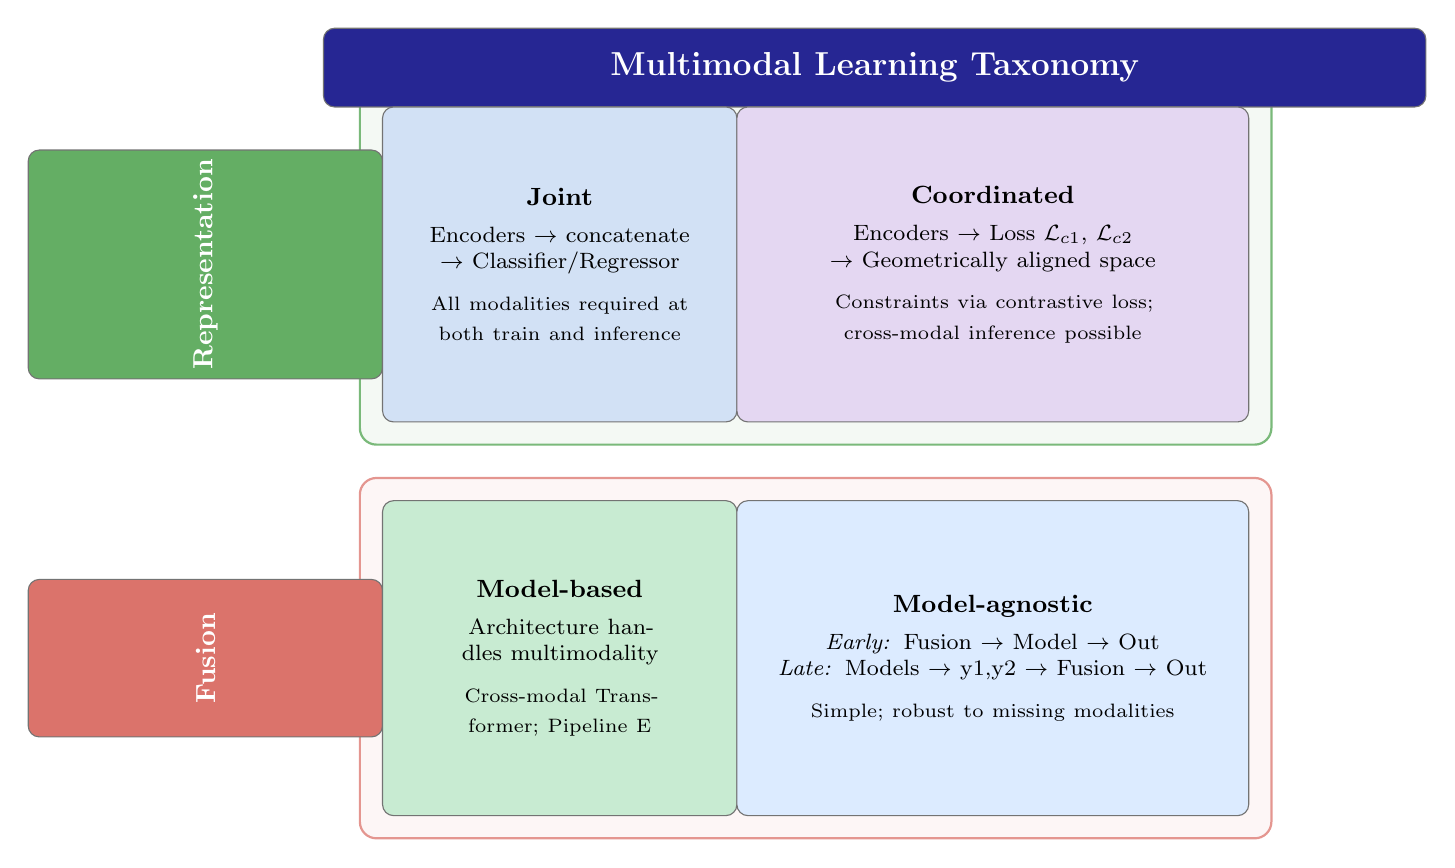
\begin{tikzpicture}[node distance=0.7cm and 1.1cm]
  \node[basebox,fill=NavyBlue!85,text=white,minimum width=14cm,minimum height=1cm,font=\large\bfseries] (hdr)
      at (0,0) {Multimodal Learning Taxonomy};

  \node[basebox,fill=ForestGreen!70,text=white,minimum width=2.0cm,minimum height=4.5cm,
        font=\bfseries,rotate=90,anchor=center] (repLabel) at (-8.5,-2.5) {Representation};
  \node[basebox,fill=coralred!80,text=white,minimum width=2.0cm,minimum height=4.5cm,
        font=\bfseries,rotate=90,anchor=center] (fusLabel) at (-8.5,-7.5) {Fusion};

  \node[basebox,fill=boxblue,minimum width=4.5cm,minimum height=4.0cm,
        text width=4.2cm] (joint) at (-4,-2.5)
      {\textbf{Joint}\\[4pt]
       \footnotesize Encoders $\to$ concatenate\\
       $\to$ Classifier/Regressor\\[4pt]
       \scriptsize All modalities required at both train and inference};

  \node[basebox,fill=boxpurple,minimum width=6.5cm,minimum height=4.0cm,
        text width=6.2cm] (coord) at (1.5,-2.5)
      {\textbf{Coordinated}\\[4pt]
       \footnotesize Encoders $\to$ Loss $\mathcal{L}_{c1}$, $\mathcal{L}_{c2}$\\
       $\to$ Geometrically aligned space\\[4pt]
       \scriptsize Constraints via contrastive loss; cross-modal inference possible};

  \node[basebox,fill=boxgreen,minimum width=4.5cm,minimum height=4.0cm,
        text width=4.2cm] (modelbased) at (-4,-7.5)
      {\textbf{Model-based}\\[4pt]
       \footnotesize Architecture handles multimodality\\[4pt]
       \scriptsize Cross-modal Transformer; Pipeline E};

  \node[basebox,fill=lightblue,minimum width=6.5cm,minimum height=4.0cm,
        text width=6.2cm] (modelagnostic) at (1.5,-7.5)
      {\textbf{Model-agnostic}\\[4pt]
       \footnotesize \textit{Early:} Fusion $\to$ Model $\to$ Out\\
       \textit{Late:} Models $\to$ y1,y2 $\to$ Fusion $\to$ Out\\[4pt]
       \scriptsize Simple; robust to missing modalities};

  \begin{pgfonlayer}{background}
    \node[rectangle,draw=ForestGreen!60,fill=ForestGreen!5,rounded corners=6pt,thick,
          fit=(joint)(coord),inner sep=8pt] {};
    \node[rectangle,draw=coralred!60,fill=coralred!5,rounded corners=6pt,thick,
          fit=(modelbased)(modelagnostic),inner sep=8pt] {};
  \end{pgfonlayer}
\end{tikzpicture}
}
\caption{Complete multimodal learning taxonomy. Top row (green): representation strategies. Bottom row (red): fusion strategies. MIVA-KNIGHT employs all four cells across its five pipelines.}
\label{fig:taxonomy_overview}
\end{figure}

\subsection{Joint Multi-Modal Representations}

Joint representations concatenate modality-specific encodings before a downstream task head.

\begin{definition}[Joint Representation]
Given modalities $\mathcal{M} = \{M_1, M_2, \ldots, M_K\}$ with encoder functions $f_k : \mathcal{X}_k \to \R^{d_k}$, the joint representation is:
\[
  \mathbf{r}_{\text{joint}} = \phi\!\left(\mathbf{e}_1, \mathbf{e}_2, \ldots, \mathbf{e}_K\right), \qquad \mathbf{e}_k = f_k(x_k)
\]
where $\phi$ is a pooling function (concatenation, element-wise sum, average, etc.).
\end{definition}

\begin{axiom}[Joint Representation Completeness]
A joint representation is \emph{complete} if $\phi$ is injective with respect to the modality tuple $(\mathbf{e}_1,\ldots,\mathbf{e}_K)$, i.e., distinct modality combinations produce distinct joint representations.
\end{axiom}

\begin{theorem}[Expressiveness of Concatenation]
Concatenation $\phi_{\text{cat}}(\mathbf{e}_1,\ldots,\mathbf{e}_K) = [\mathbf{e}_1;\ldots;\mathbf{e}_K] \in \R^{\sum_k d_k}$ is the maximal-rank pooling: a linear head $g_\theta$ with $g_\theta(\mathbf{r}) = W\mathbf{r} + b$ can learn arbitrary linear combinations of all modality features, while element-wise sum $\phi_{\text{sum}}$ constrains all $d_k$ to be equal and loses cross-modality interaction terms.
\end{theorem}

\begin{algorithm}[H]
\caption{Joint Multimodal Representation (Concatenation)}
\label{alg:joint_repr}
\begin{algorithmic}[1]
\Require Modality inputs $\{x_1, x_2, \ldots, x_K\}$; trained encoders $\{f_1,\ldots,f_K\}$; pooling function $\phi$; downstream head $g_\theta$
\Ensure Prediction $\hat{y}$, joint representation $\mathbf{r}$
\State \textbf{// Step 1: Encode each modality independently}
\For{$k = 1$ to $K$}
  \State $\mathbf{e}_k \gets f_k(x_k)$ \Comment{No gradient if encoder frozen}
\EndFor
\State \textbf{// Step 2: Pool representations}
\State $\mathbf{r}_{\text{joint}} \gets \phi(\mathbf{e}_1, \mathbf{e}_2, \ldots, \mathbf{e}_K)$
  \Comment{e.g., concat: $\mathbf{r} \in \R^{\sum_k d_k}$}
\State \textbf{// Step 3: Downstream task}
\State $\hat{y} \gets g_\theta(\mathbf{r}_{\text{joint}})$
\State \textbf{// Step 4 (training only): Compute loss and update $\theta$}
\If{training}
  \State $\mathcal{L} \gets \ell(\hat{y}, y)$ \Comment{Task-specific loss}
  \State $\theta \gets \theta - \eta\,\nabla_\theta \mathcal{L}$
\EndIf
\State \Return $(\hat{y},\; \mathbf{r}_{\text{joint}})$
\end{algorithmic}
\end{algorithm}

\subsection{Coordinated Multimodal Representations}

Coordinated representations learn modality-specific encodings that are \emph{aligned through a loss function}, without explicit concatenation.

\begin{definition}[Coordinated Representation via Contrastive Loss]
For modalities $M_1, M_2$ with encoders $f_1, f_2$ and positive pairs $\mathcal{P} = \{(x_1^{(i)}, x_2^{(i)})\}_{i=1}^N$:
\[
  \mathcal{L}_{\text{coord}} = \frac{1}{2}(\mathcal{L}_{c1} + \mathcal{L}_{c2})
\]
\[
  \mathcal{L}_{c1} = -\frac{1}{B}\sum_{i=1}^B \log\frac{\exp(\mathbf{e}_1^{(i)} \cdot \mathbf{e}_2^{(i)} / \tau)}{\sum_{j=1}^B \exp(\mathbf{e}_1^{(i)} \cdot \mathbf{e}_2^{(j)} / \tau)}, \quad
  \mathcal{L}_{c2} = -\frac{1}{B}\sum_{j=1}^B \log\frac{\exp(\mathbf{e}_2^{(j)} \cdot \mathbf{e}_1^{(j)} / \tau)}{\sum_{i=1}^B \exp(\mathbf{e}_2^{(j)} \cdot \mathbf{e}_1^{(i)} / \tau)}
\]
\end{definition}

\begin{lemma}[Coordinated vs.\ Joint Representations]
Coordinated representations require both modalities only during training (for the loss signal), not necessarily at inference. If $f_1$ encodes text and $f_2$ encodes images, a query may be issued via text alone and matched against pre-encoded image embeddings in the shared space. Joint representations require all modalities at inference.
\end{lemma}

\begin{algorithm}[H]
\caption{Coordinated Representation Learning (Symmetric Contrastive)}
\label{alg:coord_repr}
\begin{algorithmic}[1]
\Require Paired dataset $\mathcal{D} = \{(x_1^{(i)}, x_2^{(i)})\}_{i=1}^N$; encoders $f_1, f_2$; temperature $\tau = 0.07$
\Ensure Coordinated encoders mapping both modalities to shared $\Sph^{511}$
\For{each mini-batch $\mathcal{B} = \{(x_1^{(i)}, x_2^{(i)})\}_{i=1}^B$}
  \State $\mathbf{e}_1^{(i)} \gets f_1(x_1^{(i)})$; $\hat{\mathbf{e}}_1^{(i)} \gets \mathbf{e}_1^{(i)}/\Norm{\mathbf{e}_1^{(i)}}$ for $i=1\ldots B$
  \State $\mathbf{e}_2^{(i)} \gets f_2(x_2^{(i)})$; $\hat{\mathbf{e}}_2^{(i)} \gets \mathbf{e}_2^{(i)}/\Norm{\mathbf{e}_2^{(i)}}$ for $i=1\ldots B$
  \State $S_{ij} \gets \hat{\mathbf{e}}_1^{(i)} \cdot \hat{\mathbf{e}}_2^{(j)} / \tau$ \Comment{Similarity matrix $[B \times B]$}
  \State $\mathcal{L}_{c1} \gets -\frac{1}{B}\sum_{i=1}^B\log\frac{\exp(S_{ii})}{\sum_{j=1}^B \exp(S_{ij})}$
  \State $\mathcal{L}_{c2} \gets -\frac{1}{B}\sum_{j=1}^B\log\frac{\exp(S_{jj})}{\sum_{i=1}^B \exp(S_{ij})}$
  \State $\mathcal{L}_{\text{coord}} \gets \frac{1}{2}(\mathcal{L}_{c1} + \mathcal{L}_{c2})$
  \State $\mathcal{L}_{\text{coord}}.\text{backward()}$; step optimiser
\EndFor
\end{algorithmic}
\end{algorithm}

\subsection{Handling Missing Modalities}

\begin{definition}[Missing Modality Problem]
A sample $\mathbf{x} = (x_1, x_2, \ldots, x_K)$ has a \emph{missing modality} $M_k$ if $x_k$ is unavailable at inference time. The system must produce a valid prediction using only the available subset $\mathcal{A} \subseteq \{1,\ldots,K\}$.
\end{definition}

\begin{axiom}[Zero-Vector Missing Modality]
\label{ax:missing}
If modality $M_k$ is absent, substituting $\mathbf{e}_k = \bm{0} \in \R^{d_k}$ in a linear projection layer results in zero contribution: $W_k \bm{0} = \bm{0}$. This provides graceful degradation without injecting noise.
\end{axiom}

\begin{algorithm}[H]
\caption{Missing-Modality Robust Inference}
\label{alg:missing_modal}
\begin{algorithmic}[1]
\Require Available modalities $\mathcal{A} \subseteq \{1,\ldots,K\}$; missing modalities $\mathcal{M} = \{1,\ldots,K\}\setminus\mathcal{A}$
\Require Projection weights $\{W_k\}$; fusion function $\phi$
\Ensure Robust representation $\mathbf{r}$
\For{$k = 1$ to $K$}
  \If{$k \in \mathcal{A}$}
    \State $\mathbf{e}_k \gets f_k(x_k)$; $\hat{\mathbf{e}}_k \gets \mathbf{e}_k / \Norm{\mathbf{e}_k}$
  \Else
    \State $\hat{\mathbf{e}}_k \gets \bm{0}^d$ \Comment{Zero-token for missing modality (Axiom~\ref{ax:missing})}
  \EndIf
\EndFor
\State $\mathbf{r} \gets \phi(\hat{\mathbf{e}}_1, \ldots, \hat{\mathbf{e}}_K)$
\If{all $k \notin \mathcal{A}$}
  \State \Return \textsc{UncertaintyResponse}()
\EndIf
\State \Return $\mathbf{r}$
\end{algorithmic}
\end{algorithm}

\subsection{Model-Based Multimodal Fusion (Cross-Modal Transformer)}

\begin{definition}[Model-Based Fusion]
In model-based fusion, the joint prediction arises from a single model $\pi_\Theta : \mathcal{X}_1 \times \cdots \times \mathcal{X}_K \to \mathcal{Y}$:
\[
  \hat{y} = \pi_\Theta(x_1, x_2, \ldots, x_K)
\]
The model architecture itself (e.g., cross-modal attention) is what enables multimodal reasoning.
\end{definition}

\begin{theorem}[Cross-Modal Attention Expressiveness]
Multi-head attention with $h$ heads over $K$ modality tokens learns $h$ independent linear combinations of modality interactions. For $K=3$ modalities and $h=8$ heads, each head can specialise in a distinct pairwise relationship (text-audio, audio-video, text-video) plus higher-order combinations, without manual feature engineering.
\end{theorem}

\begin{algorithm}[H]
\caption{Model-Based Multimodal Fusion (Cross-Modal Transformer)}
\label{alg:model_based_fusion}
\begin{algorithmic}[1]
\Require Modality embeddings $\{\hat{\mathbf{e}}_k\}_{k=1}^K$, each $\in \R^d$; Transformer parameters $\Theta$
\Ensure Fused representation $\mathbf{r}_{\text{fused}} \in \R^d$
\State $X \gets \text{stack}([\hat{\mathbf{e}}_1, \hat{\mathbf{e}}_2, \ldots, \hat{\mathbf{e}}_K],\; \text{dim}=1)$ \Comment{$[B, K, d]$}
\State $X \gets X + P$ \Comment{$P \in \R^{K \times d}$ learned modality tags}
\For{layer $\ell = 1$ to $L$}
  \State $X \gets X + \MHA(\LN(X))$ \Comment{Pre-LN cross-modal attention}
  \State $X \gets X + \text{FFN}(\LN(X))$ \Comment{Pre-LN feed-forward}
\EndFor
\State $\mathbf{r}_{\text{fused}} \gets \frac{1}{K}\sum_{k=1}^K X_{:,k,:}$ \Comment{Mean-pool over modality tokens}
\State $\hat{y} \gets g_\theta(\mathbf{r}_{\text{fused}})$
\State \Return $(\hat{y}, \mathbf{r}_{\text{fused}})$
\end{algorithmic}
\end{algorithm}

\subsection{Model-Agnostic Early and Late Fusion}

\begin{definition}[Early Fusion]
Features from all modalities are combined into a single representation $\mathbf{z} = \phi_{\text{early}}(x_1, \ldots, x_K)$ before any learned model is applied:
$\hat{y} = g_\theta(\phi_{\text{early}}(x_1, \ldots, x_K))$.
\end{definition}

\begin{definition}[Late Fusion]
$K$ independent models $\{g_k\}_{k=1}^K$ each produce $\hat{y}_k = g_k(x_k)$. A fusion function combines these:
$\hat{y} = \phi_{\text{late}}(\hat{y}_1, \ldots, \hat{y}_K)$.
Common choices: mean, weighted mean, learned MLP combiner.
\end{definition}

\begin{lemma}[Early Fusion Trade-off]
Early fusion achieves the lowest inference latency (single forward pass) but requires all modalities to be present and aligned. Missing modalities cannot be trivially handled without imputation.
\end{lemma}

\begin{proposition}[Late Fusion Missing-Modality Robustness]
Late fusion is the most robust to missing modalities: if $M_k$ is absent, the weight $w_k$ can be set to zero and the remaining modalities re-normalised: $\hat{y} = \frac{\sum_{k \in \mathcal{A}} w_k \hat{y}_k}{\sum_{k \in \mathcal{A}} w_k}$, requiring no architectural changes.
\end{proposition}

%%
%% ============================================================
%% PART IV — THE FIVE MML CHALLENGES
%% ============================================================
%%
\newpage
\section{The Five Multimodal Machine Learning Challenges}
\label{sec:fivechallenges}

\begin{tcolorbox}[keybox,title={Five Canonical MML Challenges in MIVA-KNIGHT}]
\begin{tabular}{lll}
\toprule
\textbf{Challenge} & \textbf{Core Problem} & \textbf{MIVA-KNIGHT Realisation} \\
\midrule
1.~Representation & Encode $\MA, \MB \to$ shared space & $\Sph^{511}$, InfoNCE, Pipelines A--D \\
2.~Translation & $\MA \to \MB$ mapping & Whisper STT, gTTS TTS, LLM captioning \\
3.~Fusion & Combine modalities $\to$ prediction & Cross-modal Transformer, Pipeline E \\
4.~Co-learning & Transfer knowledge between modalities & ROCO surgical transfer (2.23\%) \\
5.~Alignment & Segment $\MA$ $\leftrightarrow$ segment $\MB$ & CMU-MOSI temporal attention alignment \\
\bottomrule
\end{tabular}
\end{tcolorbox}

\subsection{Challenge 1: Multimodal Representation}

\begin{tcolorbox}[challengebox,title={Challenge 1: Representation}]
\textbf{Core question}: How do we represent modalities $\MA$ and $\MB$ so that semantically related content from each modality maps to nearby points in a shared vector space?
\end{tcolorbox}

\begin{definition}[Multimodal Representation Problem]
Given modalities $\MA$ and $\MB$ with raw data spaces $\mathcal{X}_A$ and $\mathcal{X}_B$, the representation problem is to learn encoder functions $f_A : \mathcal{X}_A \to \R^d$ and $f_B : \mathcal{X}_B \to \R^d$ such that for matching pairs:
\[
  \text{sim}(f_A(x_A^{(i)}), f_B(x_B^{(i)})) \gg \text{sim}(f_A(x_A^{(i)}), f_B(x_B^{(j)})) \quad \forall\; j \ne i.
\]
\end{definition}

\begin{definition}[Symmetric InfoNCE Loss]
For batch size $B$, temperature $\tau = 0.07$, similarity $S_{ij} = \hat{e}_A^{(i)} \cdot \hat{e}_B^{(j)} / \tau$:
\[
  \mathcal{L}_{\text{InfoNCE}} = \frac{1}{2}\left[
    -\frac{1}{B}\sum_i \log\frac{e^{S_{ii}}}{\sum_j e^{S_{ij}}}
    -\frac{1}{B}\sum_j \log\frac{e^{S_{jj}}}{\sum_i e^{S_{ij}}}
  \right]
\]
\end{definition}

\begin{theorem}[InfoNCE as Mutual Information Bound]
\[
  I(f_A(x_A);\, f_B(x_B)) \ge \log B - \mathcal{L}_{\text{InfoNCE}}
\]
Minimising $\mathcal{L}_{\text{InfoNCE}}$ maximises a lower bound on the mutual information between the two modality representations.
\end{theorem}

\begin{lemma}[Random Baseline Loss]
At random initialisation, $\EE[\mathcal{L}_{\text{InfoNCE}}] = \log B$. For $B = 32$: $\log 32 \approx 3.47$.
\end{lemma}

\begin{theorem}[Representation Quality Upper Bound]
For any encoder $f_A$ and paired dataset of size $N$, the achievable Precision@1 is upper-bounded by:
\[
  P@1 \le 1 - \frac{H(Y|\hat{e}_A)}{H(Y)}
\]
where $Y$ is the ground-truth match label and $H$ is entropy.
\end{theorem}

\begin{algorithm}[H]
\caption{Challenge 1 — Multimodal Representation Learning (Coordinated Embedding)}
\label{alg:repr_challenge}
\begin{algorithmic}[1]
\Require Paired dataset $\mathcal{D} = \{(x_A^{(i)}, x_B^{(i)})\}_{i=1}^N$
\Require Frozen encoders $f_A, f_B$; trainable projection heads $P_A, P_B$ (Def.~\ref{def:projmlp})
\Require Temperature $\tau = 0.07$; batch size $B$; AdamW with lr\,$= 10^{-4}$
\Ensure Trained $P_A^*, P_B^*$ embedding both modalities into shared $\Sph^{511}$
\For{epoch $= 1$ to $E$}
  \ForEach{mini-batch $\{(x_A^{(i)}, x_B^{(i)})\}_{i=1}^B$}
    \State $h_A^{(i)} \gets f_A(x_A^{(i)})$ for $i=1\ldots B$ \Comment{Frozen backbone, no grad}
    \State $h_B^{(i)} \gets f_B(x_B^{(i)})$ for $i=1\ldots B$
    \State $\hat{e}_A^{(i)} \gets P_A(h_A^{(i)}) / \Norm{P_A(h_A^{(i)})}_2 \in \Sph^{511}$
    \State $\hat{e}_B^{(i)} \gets P_B(h_B^{(i)}) / \Norm{P_B(h_B^{(i)})}_2 \in \Sph^{511}$
    \State $S_{ij} \gets \hat{e}_A^{(i)} \cdot \hat{e}_B^{(j)} / \tau \quad \forall\, i,j$ \Comment{$[B \times B]$ matrix}
    \State $\mathcal{L}_{A \to B} \gets -\frac{1}{B}\sum_i \log\frac{e^{S_{ii}}}{\sum_j e^{S_{ij}}}$
    \State $\mathcal{L}_{B \to A} \gets -\frac{1}{B}\sum_j \log\frac{e^{S_{jj}}}{\sum_i e^{S_{ij}}}$
    \State $\mathcal{L}_{\text{repr}} \gets \frac{1}{2}(\mathcal{L}_{A \to B} + \mathcal{L}_{B \to A})$
    \State optimizer.zero\_grad(); $\mathcal{L}_{\text{repr}}$.backward(); clip\_grad$(1.0)$; optimizer.step()
  \EndFor
  \State Evaluate: P@1, P@3, MRR on validation set
\EndFor
\State \Return $(P_A^*, P_B^*)$
\end{algorithmic}
\end{algorithm}

\subsection{Challenge 2: Multimodal Translation}

\begin{tcolorbox}[challengebox,title={Challenge 2: Translation}]
\textbf{Core question}: Given an observation in Modality~A, how do we generate a meaningful, accurate representation in Modality~B?
\end{tcolorbox}

\begin{definition}[Multimodal Translation]
The translation task is to generate $\hat{x}_B \in \mathcal{X}_B$ from $x_A \in \mathcal{X}_A$ such that $\hat{x}_B$ is \emph{faithful} (accurately reflects $x_A$) and \emph{fluent} (natural in $\mathcal{X}_B$).
\end{definition}

\begin{theorem}[Faithfulness vs.\ Fluency Trade-off]
For any translation model $g : \mathcal{X}_A \to \mathcal{X}_B$, expected faithfulness $F$ and fluency $Q$ satisfy:
$F \cdot Q \le \frac{1}{4}(F + Q)^2$.
Maximising one without constraint on the other produces a degenerate translator.
\end{theorem}

\begin{axiom}[Grounding Constraint]
\label{ax:grounding}
A faithful translation must be grounded: every claim in $\hat{x}_B$ must be inferable from $x_A$ or a verified knowledge source. MIVA-KNIGHT enforces this via RAG: the LLM translates retrieved context, not its parametric knowledge.
\end{axiom}

\begin{definition}[Whisper CTC-Attention Architecture]
Whisper is a seq2seq model: $P(\hat{q} \mid x_s) = \prod_{t=1}^T P(q_t \mid q_{1:t-1},\, \text{Enc}(x_s))$ where Enc is a convolutional + Transformer encoder over mel-spectrogram frames, and Dec is an autoregressive Transformer decoder.
\end{definition}

\begin{algorithm}[H]
\caption{Challenge 2 --- Multimodal Translation (Three Pathways)}
\label{alg:trans_challenge}
\begin{algorithmic}[1]
\Require Input $x$ of source modality $\MA$; target modality $\MB \in \{\text{text, image, audio}\}$
\Ensure Translation $\hat{x}_B$ in target modality $\MB$
\Procedure{Translate}{$x, \MA, \MB$}
\If{$\MA = \text{speech}$, $\MB = \text{text}$} \Comment{\textbf{Pathway 1: Speech-to-Text (STT)}}
  \State Resample $x$ to 16\,kHz mono; compute log-mel spectrogram (80 bins)
  \State $\hat{q} \gets \text{Whisper.decode}(\text{mel}, \text{language}=\text{``en''})$
  \State \Return $\hat{q}$
\EndIf
\If{$\MA = \text{image}$, $\MB = \text{caption/text}$} \Comment{\textbf{Pathway 2: Image-to-Caption}}
  \State $h_I \gets \text{ResNet50}(x)$ \Comment{pool5 features $[2048]$}
  \State $\hat{e}_I \gets P_I(h_I) / \Norm{P_I(h_I)}_2 \in \Sph^{511}$
  \State $\mathcal{D}^* \gets \text{HybridRetriever.retrieve}(\hat{e}_I)$
  \State $\Pi \gets$ ``Describe the image using ONLY these captions: $\mathcal{D}^*$''
  \State $\hat{x}_B \gets \text{LLM.generate}(\Pi)$
  \State \Return $\hat{x}_B$
\EndIf
\If{$\MA = \text{text}$, $\MB = \text{audio}$} \Comment{\textbf{Pathway 3: Text-to-Speech (TTS)}}
  \State buf $\gets$ BytesIO(); $\text{gTTS}(x).\text{write\_to\_fp}(\text{buf})$; buf.seek(0)
  \State \Return buf.read() \Comment{MP3 bytes, no disk I/O}
\EndIf
\EndProcedure
\end{algorithmic}
\end{algorithm}

\subsection{Challenge 3: Multimodal Fusion}

\begin{tcolorbox}[challengebox,title={Challenge 3: Fusion}]
\textbf{Core question}: How do we combine signals from multiple modalities to make a single prediction that outperforms any single-modality model?
\end{tcolorbox}

\begin{definition}[Multimodal Fusion Problem]
Given embeddings $\eA \in \R^{d_A}$ and $\eB \in \R^{d_B}$, learn $g : \R^{d_A} \times \R^{d_B} \to \mathcal{Y}$ outperforming any unimodal predictor.
\end{definition}

\begin{axiom}[Fusion Benefit]
\label{ax:fusion}
Fusion is beneficial iff the modalities are \emph{complementary}: $I((\eA, \eB); Y) > \max(I(\eA; Y), I(\eB; Y))$.
\end{axiom}

\begin{definition}[Multi-Task Fusion Loss --- Pipeline E]
\[
  \mathcal{L}_{\text{fusion}}(\hat{y}, y, b) = 0.6 \cdot \mathcal{L}_{\text{MSE}}(\hat{y}, y) + 0.4 \cdot \mathcal{L}_{\text{BCE}}(\hat{y}, b)
\]
where $y \in [-3,+3]$ (regression), $b \in \{0,1\}$ (binary).
\end{definition}

\begin{theorem}[Stable BCE with Logits]
\[
  \mathcal{L}_{\text{BCE}}(\hat{y}, b) = \max(0, \hat{y}) - b\hat{y} + \log(1 + e^{-|\hat{y}|})
\]
This numerically stable form avoids overflow in $e^{\hat{y}}$ for large positive $\hat{y}$.
\end{theorem}

\begin{algorithm}[H]
\caption{Challenge 3 --- Multimodal Fusion (Cross-Modal Transformer, Pipeline E)}
\label{alg:fusion_challenge}
\begin{algorithmic}[1]
\Require Modality embeddings $\hat{e}_1, \hat{e}_2, \ldots, \hat{e}_K \in \R^{512}$; parameters $\theta$
\Require Ground-truth $y$ (continuous), $b$ (binary)
\Ensure Prediction $\hat{y}$; loss $\mathcal{L}_{\text{fusion}}$
\State $X \gets \text{stack}([\hat{e}_1,\ldots,\hat{e}_K], \text{dim}=1) \in \R^{B \times K \times 512}$
\State $X \gets X + P$ \Comment{Learnable modality positional encodings}
\For{$\ell = 1$ to $L=2$}
  \State $X \gets X + \MHA(\LN(X))$ \Comment{Pre-LN self-attention across all modalities}
  \State $X \gets X + \text{FFN}(\LN(X))$
\EndFor
\State $\bar{x} \gets X.\text{mean(dim=1)} \in \R^{B \times 512}$
\State $\hat{y} \gets W_2(\GELU(W_1 \bar{x})) \in \R^B$ \Comment{$512 \to 256 \to 1$}
\State $\mathcal{L}_{\text{MSE}} \gets \frac{1}{B}\sum({\hat{y} - y})^2$
\State $\mathcal{L}_{\text{BCE}} \gets \text{binary\_cross\_entropy\_with\_logits}(\hat{y}, b)$
\State $\mathcal{L}_{\text{fusion}} \gets 0.6 \cdot \mathcal{L}_{\text{MSE}} + 0.4 \cdot \mathcal{L}_{\text{BCE}}$
\State optimizer.zero\_grad(); $\mathcal{L}_{\text{fusion}}$.backward(); optimizer.step()
\State \Return $(\hat{y}, \mathcal{L}_{\text{fusion}})$
\end{algorithmic}
\end{algorithm}

\subsection{Challenge 4: Co-learning}

\begin{tcolorbox}[challengebox,title={Challenge 4: Co-learning}]
\textbf{Core question}: How can a strong modality help train a weaker modality, especially when the weaker modality has limited labelled data?
\end{tcolorbox}

\begin{definition}[Surgical Co-learning Transfer]
\label{def:surgical}
Given source domain $\mathcal{D}_{\text{src}}$ (COCO, trained) and target domain $\mathcal{D}_{\text{tgt}}$ (ROCO, new), surgical transfer trains only the domain-specific projection head $P_I^{\text{tgt}}$:
\[
  \phi^* = \argmin_\phi \mathcal{L}_{\text{co}}(\phi) = \mathcal{L}_{\text{InfoNCE}}(P_I^\phi \circ f_I, f_T) + \lambda \mathcal{L}_{\text{distill}}(\phi)
\]
\[
  \mathcal{L}_{\text{distill}}(\phi) = \frac{1}{B}\sum_{i=1}^B \Norm{f_T^{\text{tgt}}(c_i) - f_T^{\text{src}}(c_i)}_2^2
\]
\end{definition}

\begin{theorem}[Surgical Transfer Efficiency]
Under Definition~\ref{def:surgical}, only $5.25\,\text{M}$ out of $235.15\,\text{M}$ total parameters are modified:
\[
  \eta_{\text{surgical}} = \frac{5.25}{235.15} \approx 2.23\%.
\]
\end{theorem}

\begin{axiom}[Minimal Retraining Principle]
Only the module responsible for translating domain-specific features into the shared embedding space (ImageProjection) is retrained per domain. All upstream encoders serve as immutable feature extractors.
\end{axiom}

\begin{lemma}[Domain Swap Isolation]
Replacing $P_I^{\text{src}} \to P_I^{\text{tgt}}$ does not move existing text or audio embeddings in $\Sph^{511}$. Medical domain transfer cannot degrade general-domain text retrieval.
\end{lemma}

\subsection{Challenge 5: Multimodal Alignment}

\begin{tcolorbox}[challengebox,title={Challenge 5: Alignment}]
\textbf{Core question}: How do we find corresponding sub-elements of $\MA$ and $\MB$ without explicit supervision of the correspondence?
\end{tcolorbox}

\begin{definition}[Multimodal Alignment Problem]
Given sequences $X_A = [x_A^{(1)},\ldots,x_A^{(T_A)}]$ and $X_B = [x_B^{(1)},\ldots,x_B^{(T_B)}]$, the alignment problem is to find a mapping $\alpha : \{1,\ldots,T_A\} \to \{1,\ldots,T_B\}$ such that $x_A^{(t)}$ and $x_B^{(\alpha(t))}$ correspond semantically.
\end{definition}

\begin{theorem}[Attention as Soft Alignment]
In the cross-modal Transformer of Pipeline E, the attention matrix $\text{Attn}(Q, K, V)_{ti'} = \frac{\exp(Q_t \cdot K_{t'}/\sqrt{d_k})}{\sum_{t''}\exp(Q_t \cdot K_{t''}/\sqrt{d_k})}$ provides a soft differentiable alignment between audio waveform segments (rows) and text tokens (columns) in the CMU-MOSI dataset.
\end{theorem}

\begin{algorithm}[H]
\caption{Challenge 5 --- Temporal Alignment via Cross-Modal Attention (CMU-MOSI)}
\label{alg:alignment_challenge}
\begin{algorithmic}[1]
\Require Audio segments $\{e_A^{(t)}\}_{t=1}^{T_A}$; text tokens $\{e_T^{(t')}\}_{t'=1}^{T_B}$; attention heads $h$
\Ensure Soft alignment matrix $\text{Align} \in \R^{T_A \times T_B}$; sentiment $\hat{y}$
\State Stack tokens: $X \gets [e_T^{(1)},\ldots,e_T^{(T_B)}, e_A^{(1)},\ldots,e_A^{(T_A)}] \in \R^{(T_A+T_B) \times 512}$
\State $Q \gets XW^Q$; $K \gets XW^K$; $V \gets XW^V$ \Comment{Project to head dimension $d_k = 64$}
\State $\text{Attn} \gets \softmax(QK^\top / \sqrt{d_k}) \in \R^{(T_A+T_B) \times (T_A+T_B)}$
\State $\text{Align} \gets \text{Attn}[T_B{:},\; :T_B]$ \Comment{Audio-to-text sub-block}
\State \Comment{Each row: how much attention audio segment $t$ pays to each text token $t'$}
\State $Z \gets \text{Attn} \cdot V$; mean-pool; regression head $\to \hat{y}$
\State \Return $(\text{Align}, \hat{y})$
\end{algorithmic}
\end{algorithm}

%%
%% ============================================================
%% PART V — PIPELINE A: GENERAL DOMAIN (COCO)
%% ============================================================
%%
\newpage
\section{Pipeline A: General Domain --- COCO Text-Image Retrieval}
\label{sec:pipelineA}

\subsection{Overview}

Pipeline~A trains a coordinated multimodal embedding on the COCO val2017 dataset (202,654 image-caption pairs) using symmetric InfoNCE loss, building the foundation for the shared $\Sph^{511}$ space.

\begin{figure}[H]
\centering
\resizebox{\textwidth}{!}{%
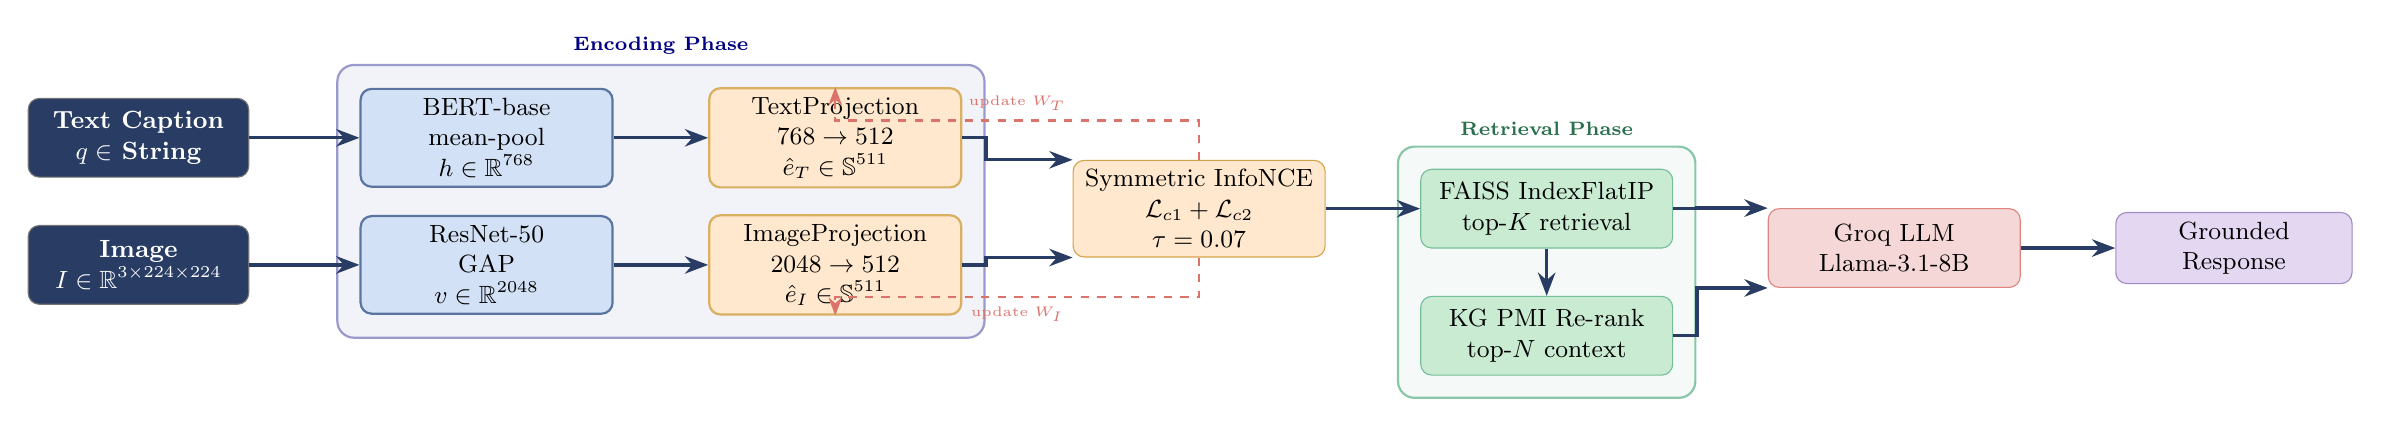
\begin{tikzpicture}[node distance=0.7cm and 1.0cm]
  \node[inputnode] (textq) at (0,0) {Text Caption\\$q \in$ String};
  \node[inputnode,below=0.6cm of textq] (imgq) {Image\\$I \in \R^{3\times224\times224}$};

  \node[encnode,right=1.4cm of textq] (bert) {BERT-base\\mean-pool\\$h \in \R^{768}$};
  \node[encnode,right=1.4cm of imgq] (resnet) {ResNet-50\\GAP\\$v \in \R^{2048}$};

  \node[projnode,right=1.2cm of bert] (tproj) {TextProjection\\$768 \to 512$\\$\hat{e}_T \in \Sph^{511}$};
  \node[projnode,right=1.2cm of resnet] (iproj) {ImageProjection\\$2048 \to 512$\\$\hat{e}_I \in \Sph^{511}$};

  \node[lossnode,right=1.4cm of tproj,yshift=-0.9cm] (loss) {Symmetric InfoNCE\\$\mathcal{L}_{c1} + \mathcal{L}_{c2}$\\$\tau = 0.07$};

  \node[retnode,right=1.2cm of loss] (faiss) {FAISS IndexFlatIP\\top-$K$ retrieval};
  \node[retnode,below=0.6cm of faiss] (kg) {KG PMI Re-rank\\top-$N$ context};
  \node[gennode,right=1.2cm of faiss,yshift=-0.5cm] (llm) {Groq LLM\\Llama-3.1-8B};
  \node[outnode,right=1.2cm of llm] (out) {Grounded\\Response};

  \draw[thickarr] (textq)--(bert); \draw[thickarr] (imgq)--(resnet);
  \draw[thickarr] (bert)--(tproj); \draw[thickarr] (resnet)--(iproj);
  \draw[thickarr] (tproj.east) -- ++(0.3,0) |- (loss.north west);
  \draw[thickarr] (iproj.east) -- ++(0.3,0) |- (loss.south west);
  \draw[redarr,dashed] (loss.north) -- ++(0,0.5) -| (tproj.north)
      node[near start,above,font=\tiny]{update $W_T$};
  \draw[redarr,dashed] (loss.south) -- ++(0,-0.5) -| (iproj.south)
      node[near start,below,font=\tiny]{update $W_I$};
  \draw[thickarr] (loss.east) -- ++(0.3,0) |- (faiss.west);
  \draw[thickarr] (faiss.south)--(kg.north);
  \draw[thickarr] (faiss.east) -- ++(0.3,0) |- (llm.north west);
  \draw[thickarr] (kg.east) -- ++(0.3,0) |- (llm.south west);
  \draw[thickarr] (llm)--(out);

  \begin{pgfonlayer}{background}
    \node[rectangle,draw=NavyBlue!40,fill=NavyBlue!5,rounded corners=6pt,thick,
          fit=(bert)(resnet)(tproj)(iproj),inner sep=8pt,
          label={[font=\scriptsize\bfseries,color=NavyBlue]above:Encoding Phase}] {};
    \node[rectangle,draw=mintgreen!60,fill=mintgreen!5,rounded corners=6pt,thick,
          fit=(faiss)(kg),inner sep=8pt,
          label={[font=\scriptsize\bfseries,color=mintgreen!70!black]above:Retrieval Phase}] {};
  \end{pgfonlayer}
\end{tikzpicture}
}
\caption{Pipeline~A architecture: COCO text-image coordinated embedding with two-stage RAG retrieval.}
\label{fig:pipeline_a}
\end{figure}

\subsection{Text Encoder: BERT Mean-Pool + TextProjection}

\begin{definition}[TextProjection $f_T$]
$f_T : \R^{768} \to \Sph^{511}$ defined by Definition~\ref{def:projmlp} with $d_{\text{in}} = 768$. Trainable parameters: $\approx$1.6\,M.
\end{definition}

\begin{remark}[Mean Pooling vs.\ CLS]
CLS token ($H_{:,0,:}$) is optimised for classification but degrades for long sequences. Mean pooling ($\frac{1}{T}\sum H_{:,t,:}$) provides better semantic similarity for retrieval tasks (consistent with sentence-transformers literature).
\end{remark}

\begin{algorithm}[H]
\caption{TextEncoderV2.encode --- BERT Mean-Pool + TextProjection}
\label{alg:textencode}
\begin{algorithmic}[1]
\Require Text $t \in$ String; frozen BERT; trained TextProjection $P_\theta$ (Def.~\ref{def:projmlp}, $d_{\text{in}}=768$)
\Ensure $e_q \in \Sph^{511}$, entity set $\mathcal{E}_q$, domain hint
\State \textbf{Tokenise:} $\text{tokens} \gets \text{WordPiece}(t, \texttt{max\_length}=128, \texttt{truncation=True})$
\State \textbf{BERT forward} (no grad):
  $H \gets \text{BERT}(\text{tokens}).\text{last\_hidden\_state} \in \R^{1 \times T \times 768}$
\State \textbf{Mean pool:} $h_{\text{BERT}} \gets \frac{1}{T}\sum_{t=1}^T H_{:,t,:} \in \R^{768}$
\State \textbf{Project:} $e_{\text{raw}} \gets P_\theta(h_{\text{BERT}}) \in \R^{512}$
\State \textbf{Normalise:} $e_q \gets e_{\text{raw}} / \Norm{e_{\text{raw}}}_2$
\State \textbf{NER:} $\mathcal{E}_q \gets \{\text{noun chunks}\} \cup \{\text{named entities}\}$ (lowercased)
\State domain\_hint $\gets$ ``medical'' if $|\{w \in \textsc{Medical\_Terms} : w \subseteq t.\text{lower}()\}| \ge 2$ else None
\State \Return $(e_q,\; \mathcal{E}_q,\; \text{domain\_hint})$
\end{algorithmic}
\end{algorithm}

\subsection{Image Encoder: ResNet-50 + ImageProjection}

\begin{definition}[ImageProjection $f_\phi$]
\[
  f_\phi : \R^{2048} \to \Sph^{511}, \qquad
  f_\phi(x) = \frac{g_\phi(x)}{\Norm{g_\phi(x)}_2}
\]
\[
  g_\phi(x) = \LN_{512}\!\left(W_2 \cdot \GELU(\LN_{2048}(W_1 x + b_1)) + b_2\right)
\]
where $W_1 \in \R^{2048 \times 2048}$, $W_2 \in \R^{512 \times 2048}$. Total: $\approx$5.25\,M parameters.
\end{definition}

\begin{axiom}[Mandatory ImageNet Normalisation]
Input images must be normalised per channel:
\[
  \hat{x}_{c,h,w} = \frac{x_{c,h,w} - \mu_c}{\sigma_c}, \quad
  \bm{\mu} = [0.485, 0.456, 0.406], \quad \bm{\sigma} = [0.229, 0.224, 0.225].
\]
ResNet-50 BatchNorm layers are calibrated with these statistics; deviations degrade pool5 features.
\end{axiom}

\begin{algorithm}[H]
\caption{Pipeline A Training Epoch (Symmetric InfoNCE)}
\label{alg:trainepoch_A}
\begin{algorithmic}[1]
\Require COCO DataLoader $L$; TextProjection $P_\theta$; ImageProjection $f_\phi$; $\tau = 0.07$
\Ensure Updated $P_\theta, f_\phi$; epoch loss
\State total\_loss $\gets 0$
\ForEach{batch $(I^{B \times 3 \times 224 \times 224},\; T^B)$ in $L$}
  \State $\hat{e}_T^{(b)} \gets \textsc{TextEncoderV2}(T[b])$ for $b=1\ldots B$ \quad $\Rightarrow E_T \in \R^{B \times 512}$
  \State $\hat{e}_I^{(b)} \gets f_\phi(\text{ResNet50}(I[b]))$ for $b=1\ldots B$ \quad $\Rightarrow E_I \in \R^{B \times 512}$
  \State $S \gets E_T \cdot E_I^\top \in \R^{B \times B}$; \quad $\mathcal{L} \gets \mathcal{L}_{\text{InfoNCE}}(E_T, E_I, \tau)$
  \State optimizer.zero\_grad(); $\mathcal{L}$.backward()
  \State clip\_grad\_norm$(\nabla\theta, c=1.0)$; optimizer.step(); scheduler.step()
  \State total\_loss $\mathrel{+}= \mathcal{L}$.item()
\EndFor
\State \Return total\_loss / $|L|$
\end{algorithmic}
\end{algorithm}

%%
%% ============================================================
%% PART VI — KNOWLEDGE GRAPH CONSTRUCTION
%% ============================================================
%%
\newpage
\section{Knowledge Graph: PMI-Weighted Entity Graph}
\label{sec:kg}

\begin{definition}[General Knowledge Graph $\KG_G$]
\[
  \KG_G = (\mathcal{V}_G, \mathcal{E}_G, w), \quad
  \mathcal{V}_G = \text{top-2000 COCO entities (spaCy)}, \quad
  (a,b) \in \mathcal{E}_G \Leftrightarrow \text{PMI}(a,b) > 0.
\]
\[
  \text{PMI}(a,b) = \log\frac{c_{ab} \cdot N}{f_a \cdot f_b + \varepsilon}, \quad w(a,b) = \text{PMI}(a,b).
\]
\end{definition}

\begin{axiom}[PMI Semantic Association]
$\text{PMI}(a,b) > 0 \Leftrightarrow$ entities $a, b$ co-occur more than expected under independence.
\end{axiom}

\begin{algorithm}[H]
\caption{Build NER Knowledge Graph (PMI-Weighted)}
\label{alg:kg_build}
\begin{algorithmic}[1]
\Require $N$ captions; spaCy \texttt{en\_core\_web\_sm}; top-$V = 2000$ entities
\Ensure \texttt{ner\_kg.pkl}: $\text{dict}[\text{entity} \to \text{dict}[\text{entity} \to \text{PMI}]]$
\For{captions in batches of 1,000}
  \State $\mathcal{E}_{\text{doc}} \gets \{\text{noun chunks}\} \cup \{\text{named entities}\}$ (lowercased)
  \State Append to all\_doc\_entities
\EndFor
\State entity\_freq $\gets \text{Counter}(\bigcup \mathcal{E}_{\text{doc}})$
\State $\mathcal{V}_G \gets \text{top-}V$ entities with freq $\ge 5$
\For{each document entity set $E_i$ (filtered to $\mathcal{V}_G$)}
  \For{each symmetric pair $(a,b) \in E_i \times E_i,\; a \ne b$}
    \State cooc$[a][b] \mathrel{+}= 1$; cooc$[b][a] \mathrel{+}= 1$
  \EndFor
\EndFor
\For{each $a \in \mathcal{V}_G$ with freq $\ge 5$}
  \For{each $(b, c_{ab})$ with $c_{ab} \ge 3$}
    \State $\text{pmi} \gets \log(c_{ab} \cdot N / (f_a \cdot f_b + \varepsilon))$
    \If{pmi $> 0$} $\KG_G[a][b] \gets \text{pmi}$ \EndIf
  \EndFor
\EndFor
\State \texttt{pickle.dump}($\KG_G$)
\end{algorithmic}
\end{algorithm}

\begin{algorithm}[H]
\caption{KG Depth-First Neighbour Search (max-2-hop)}
\label{alg:kgdfs}
\begin{algorithmic}[1]
\Require Entity $v$, KG $\KG$, max\_hops $= 2$
\Ensure Neighbour list with PMI weights
\State visited $\gets \emptyset$; neighbours $\gets []$
\State \Call{DFS}{$v$, 1}
\Procedure{DFS}{current, hops}
  \If{hops $>$ max\_hops \textbf{or} current $\in$ visited} \Return \EndIf
  \State visited $\gets$ visited $\cup$ \{current\}
  \ForEach{$(h, r, t) \in \KG$.relationships}
    \If{$h = $ current} neighbours.append$(h, r, t, \text{hops})$; \Call{DFS}{$t$, hops+1} \EndIf
    \If{$t = $ current} neighbours.append$(t, r_{\text{inv}}, h, \text{hops})$; \Call{DFS}{$h$, hops+1} \EndIf
  \EndFor
\EndProcedure
\end{algorithmic}
\end{algorithm}

%%
%% ============================================================
%% PART VII — PIPELINE B: MEDICAL DOMAIN TRANSFER (ROCO)
%% ============================================================
%%
\newpage
\section{Pipeline B: Medical Domain Transfer --- ROCO Radiology}
\label{sec:pipelineB}

\subsection{Core Thesis: Surgical Domain Transfer}

\begin{definition}[Domain Transfer]
Let $\Sph^{511}$ be the shared embedding space from Pipeline~A, where TextProjection $f_T$ maps captions. Domain transfer trains $f_I^{\text{ROCO}}$ such that:
\[
  f_I^{\text{ROCO}}\!\left(\text{ResNet}(\text{X-ray}_i)\right) \approx f_T(\text{caption}_i), \quad \forall i \in \text{ROCO train},
\]
without moving existing text embeddings.
\end{definition}

\begin{figure}[H]
\centering
\resizebox{0.95\textwidth}{!}{%
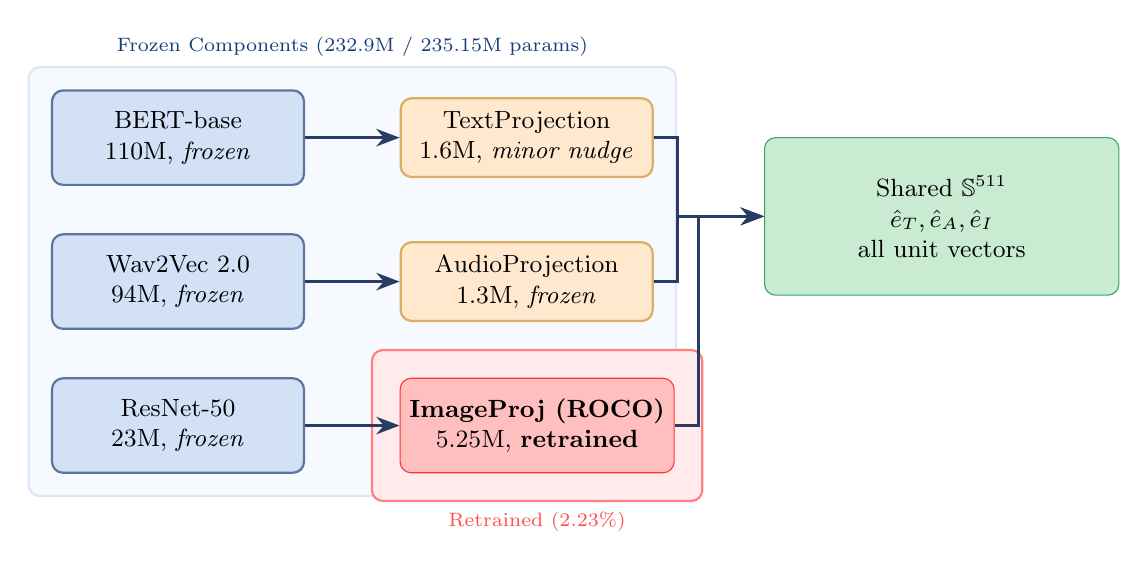
\begin{tikzpicture}[node distance=0.6cm and 1.0cm]
  \node[encnode,minimum width=3.2cm,minimum height=1.2cm] (bert) {BERT-base\\110M, \textit{frozen}};
  \node[encnode,minimum width=3.2cm,minimum height=1.2cm,below=0.6cm of bert] (wav2vec) {Wav2Vec 2.0\\94M, \textit{frozen}};
  \node[encnode,minimum width=3.2cm,minimum height=1.2cm,below=0.6cm of wav2vec] (resnet) {ResNet-50\\23M, \textit{frozen}};

  \node[projnode,minimum width=3.2cm,right=1.2cm of bert] (tproj) {TextProjection\\1.6M, \textit{minor nudge}};
  \node[projnode,minimum width=3.2cm,right=1.2cm of wav2vec] (aproj) {AudioProjection\\1.3M, \textit{frozen}};
  \node[basebox,fill=red!25,draw=red!80,minimum width=3.2cm,minimum height=1.2cm,
        right=1.2cm of resnet] (iproj) {\textbf{ImageProj (ROCO)}\\5.25M, \textbf{retrained}};

  \node[basebox,fill=boxgreen,draw=mintgreen,minimum width=4.5cm,minimum height=2.0cm,
        right=1.4cm of tproj,yshift=-1.0cm] (shared) {Shared $\Sph^{511}$\\$\hat{e}_T, \hat{e}_A, \hat{e}_I$\\all unit vectors};

  \draw[thickarr] (bert)--(tproj); \draw[thickarr] (wav2vec)--(aproj); \draw[thickarr] (resnet)--(iproj);
  \draw[thickarr] (tproj.east) -- ++(0.3,0) |- (shared.west);
  \draw[thickarr] (aproj.east) -- ++(0.3,0) |- (shared.west);
  \draw[thickarr] (iproj.east) -- ++(0.3,0) |- (shared.west);

  \begin{pgfonlayer}{background}
    \node[rectangle,draw=boxblue!80,fill=boxblue!20,rounded corners,thick,
          fit=(bert)(wav2vec)(resnet)(tproj)(aproj),inner sep=8pt,
          label={[font=\scriptsize,color=navyblue]above:Frozen Components (232.9M / 235.15M params)}] {};
    \node[rectangle,draw=red!50,fill=red!8,rounded corners,thick,
          fit=(iproj),inner sep=10pt,
          label={[font=\scriptsize,color=red!70]below:Retrained (2.23\%)}] {};
  \end{pgfonlayer}
\end{tikzpicture}
}
\caption{Pipeline~B surgical domain transfer: only ImageProjection (5.25M/235M params) is retrained for ROCO medical domain.}
\label{fig:pipeline_b}
\end{figure}

\begin{definition}[Dual Loss with Knowledge Distillation]
\[
  \mathcal{L}_{\text{total}} = \mathcal{L}_{\text{align}} + \lambda(t) \cdot \mathcal{L}_{\text{distill}}
\]
\[
  \mathcal{L}_{\text{distill}} = \frac{1}{B}\sum_{i=1}^B \Norm{f_T^{\text{ROCO}}(c_i) - f_T^{\text{M2}}(c_i)}_2^2
\]
where $\lambda(t)$ decays during training to prevent catastrophic forgetting.
\end{definition}

\begin{theorem}[RadLex Seed Coverage Guarantee]
By forcing all RadLex seed terms into $\mathcal{V}_M$, critical imaging terms (e.g.\ \emph{pneumothorax}, \emph{cardiomegaly}) are guaranteed to appear in $\KG_M$ even if they are rare in the ROCO validation split.
\end{theorem}

\begin{algorithm}[H]
\caption{Fine-tune ImageProjection for ROCO Medical Domain}
\label{alg:finetune_roco}
\begin{algorithmic}[1]
\Require ROCO train metadata ($\approx$60K pairs); frozen TextProjection + BERT; frozen ResNet-50
\Ensure \texttt{image\_projection\_roco.pth}
\State Init fresh ImageProjection (random weights)
\State opt$_I \gets$ AdamW(ImageProjection.params, lr=$5\times10^{-4}$)
\State opt$_T \gets$ AdamW(TextProjection.params, lr=$10^{-5}$) \Comment{Nudge only}
\For{epoch $= 1$ to $15$}
  \ForEach{batch $(c_i, \text{img\_path}_i)_{i=1}^{32}$}
    \State $\hat{e}_T \gets \text{L2-norm}(f_T(\text{BERT}(\text{tokenise}(c_i))))$ \quad $[B,512]$
    \State $\hat{e}_I \gets f_\phi(\text{ResNet}(\text{preprocess}(\text{img}_i)))$ \quad $[B,512]$
    \State $\mathcal{L} \gets \mathcal{L}_{\text{InfoNCE}}(\hat{e}_T, \hat{e}_I, \tau{=}0.07) + \lambda(t)\cdot\mathcal{L}_{\text{distill}}$
    \State $\mathcal{L}$.backward(); opt$_I$.step(); opt$_T$.step()
  \EndFor
  \State Save best checkpoint (val loss)
\EndFor
\end{algorithmic}
\end{algorithm}

%%
%% ============================================================
%% PART VIII — TWO-STAGE HYBRID RETRIEVAL
%% ============================================================
%%
\newpage
\section{Two-Stage Hybrid Retrieval Engine}
\label{sec:retrieval}

\subsection{Architecture Overview}

\begin{figure}[H]
\centering
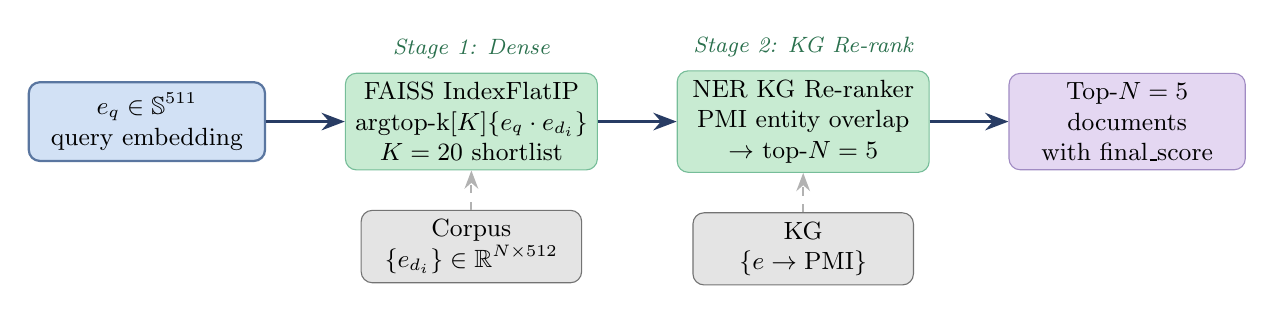
\begin{tikzpicture}[node distance=0.65cm and 1.0cm]
  \node[encnode,minimum width=3.0cm] (qemb) {$e_q \in \Sph^{511}$\\query embedding};
  \node[retnode,right=1.0cm of qemb] (faiss) {FAISS IndexFlatIP\\$\argtopk[K]\{e_q \cdot e_{d_i}\}$\\$K = 20$ shortlist};
  \node[retnode,right=1.0cm of faiss] (kgrank) {NER KG Re-ranker\\PMI entity overlap\\$\to$ top-$N=5$};
  \node[outnode,right=1.0cm of kgrank] (topn) {Top-$N = 5$\\documents\\with final\_score};
  \node[datanode,below=0.5cm of faiss] (corpus) {Corpus\\$\{e_{d_i}\} \in \R^{N \times 512}$};
  \node[datanode,below=0.5cm of kgrank] (kg) {KG\\$\{e \to \text{PMI}\}$};

  \draw[thickarr] (qemb)--(faiss); \draw[thickarr] (faiss)--(kgrank); \draw[thickarr] (kgrank)--(topn);
  \draw[dasharr] (corpus.north)--(faiss.south); \draw[dasharr] (kg.north)--(kgrank.south);
  \node[font=\footnotesize\itshape,color=mintgreen!70!black,above=0.05cm of faiss] {Stage 1: Dense};
  \node[font=\footnotesize\itshape,color=mintgreen!70!black,above=0.05cm of kgrank] {Stage 2: KG Re-rank};
\end{tikzpicture}
\caption{Two-stage hybrid retrieval: dense FAISS search followed by KG PMI re-ranking.}
\label{fig:retrieval}
\end{figure}

\subsection{Stage 1: FAISS Dense Retrieval}

\begin{definition}[FAISS IndexFlatIP]
\[
  \text{dense\_score}(q, d_i) = e_q \cdot e_{d_i} \in [-1,1], \quad
  \mathcal{R}_K = \argtopk_{i}\;(e_q \cdot e_{d_i})
\]
For $N = 69{,}866$ ROCO vectors, exact inner-product search requires $O(N \cdot d) \approx 3.6 \times 10^7$ MACs ($\approx$15\,ms CPU).
\end{definition}

\subsection{Stage 2: PMI Entity Re-ranking}

\begin{algorithm}[H]
\caption{NER KG Re-ranker (Full Algorithm)}
\label{alg:rerank}
\begin{algorithmic}[1]
\Require Shortlist $S = [d_1,\ldots,d_K]$ with dense\_score; query entities $\mathcal{E}_q$; KG; $\alpha = 0.7$
\Ensure Top-$N$ documents with final\_score $\in [0,1]$
\State $s_{\min} \gets \min_i \text{dense\_score}(d_i)$;\; $s_{\max} \gets \max_i \text{dense\_score}(d_i)$;\; $\Delta \gets \max(s_{\max}-s_{\min}, 10^{-6})$
\State $\tilde{s}_{\text{dense}}(d_i) \gets (\text{dense\_score}(d_i) - s_{\min}) / \Delta$
\ForEach{$d_i \in S$}
  \State $\mathcal{E}_{d_i} \gets \text{word-boundary regex extraction from } d_i.\text{text}$
  \State $\text{kg\_raw}(d_i) \gets \sum_{q \in \mathcal{E}_q}\sum_{d \in \mathcal{E}_{d_i}} \text{PMI}(q,d) \cdot \mathbf{1}[q \in \KG,\; d \in \KG[q]]$
\EndFor
\State $m_{\KG} \gets \max_i \text{kg\_raw}(d_i)$;\quad $\tilde{s}_{\KG}(d_i) \gets \text{kg\_raw}(d_i) / \max(m_{\KG}, 10^{-6})$
\ForEach{$d_i \in S$}
  \State $\text{final\_score}(d_i) \gets \alpha \cdot \tilde{s}_{\text{dense}}(d_i) + (1-\alpha)\cdot\tilde{s}_{\KG}(d_i)$
\EndFor
\State \Return $\text{top-}N(S,\; \text{by final\_score desc})$
\end{algorithmic}
\end{algorithm}

\begin{theorem}[Score Bounds]
$\text{final\_score}(d_i) \in [0,1]$ for all $d_i \in S$ under Algorithm~\ref{alg:rerank}, since $\tilde{s}_{\text{dense}}, \tilde{s}_{\KG} \in [0,1]$ by min-max normalisation and $\alpha + (1-\alpha) = 1$.
\end{theorem}

\begin{lemma}[KG Re-ranking Monotonicity]
Since PMI$(a,b) > 0$ is required for every edge, all KG boosts are non-negative. Re-ranking can only improve the rank of semantically related documents; it cannot demote a document below its FAISS-only rank unless another document receives a larger boost.
\end{lemma}

\subsection{Tiered Confidence Guard}

\begin{definition}[Confidence Tier Function]
\[
  \text{tier}(s) = \begin{cases}
    \texttt{full}     & s \ge \tau \\
    \texttt{partial}  & \tau - 0.2 \le s < \tau \\
    \texttt{rejected} & s < \tau - 0.2
  \end{cases}, \quad
  \tau_{\text{general}} = 0.40,\; \tau_{\text{medical}} = 0.55.
\]
\end{definition}

\begin{axiom}[Clinical Safety Constraint]
For clinical domains, false positives carry higher risk than false negatives:
$\tau_{\text{medical}} = \tau_{\text{general}} + 0.15$. The system prefers refusing to answer over generating a plausible but unsafe medical hallucination.
\end{axiom}

\begin{algorithm}[H]
\caption{Full Query Pipeline --- MIVA-KNIGHT Inference}
\label{alg:query}
\begin{algorithmic}[1]
\Require user\_input: TextQuery or AudioQuery; loaded pipeline
\Ensure GeneratorOutput: answer, sources, emotion, audio (optional)
\If{user\_input is AudioQuery}
  \State (transcript, emotion, conf\_emo) $\gets$ AudioEncoder.encode$(a)$
  \If{transcript $= \varnothing$} \Return rejection \EndIf
  \State $(e_q, \mathcal{E}_q, h) \gets$ TextEncoder.encode(transcript)
\Else
  \State $(e_q, \mathcal{E}_q, h) \gets$ TextEncoder.encode$(q)$; emotion $\gets$ ``neutral''
\EndIf
\If{$h \ne \varnothing$} \Call{SwapDomain}{MedicalDomain if $h=$``medical'' else GeneralDomain} \EndIf
\State $(\mathcal{D}^*, s_{\max}) \gets$ HybridRetriever.retrieve$(e_q, \mathcal{E}_q)$
\State tier $\gets$ tier$(s_{\max})$
\If{tier $=$ ``rejected''} \Return \textsc{TieredRejection}(domain.name) \EndIf
\State $g \gets$ GeneratorInput$(q, \text{emotion}, \text{conf\_emo}, \mathcal{D}^*, \Pi, \text{tier})$
\State result $\gets$ Generator.generate$(g)$
\If{TTS enabled} result.audio $\gets$ gTTS.convert(result.answer) \EndIf
\State \Return result
\end{algorithmic}
\end{algorithm}

\begin{theorem}[RAG Faithfulness]
An answer is \emph{faithful} to retrieved context $\mathcal{D}^*$ iff every claim $c$ in the answer can be inferred from some $d_j \in \mathcal{D}^*$. MIVA-KNIGHT enforces faithfulness by: (1) prompting ``Answer using ONLY the retrieved context'', (2) requiring citation, (3) rejecting low-confidence retrievals before any LLM call.
\end{theorem}

%%
%% ============================================================
%% PART IX — PIPELINE C: RAVDESS AUDIO EMOTION
%% ============================================================
%%
\newpage
\section{Pipeline C: RAVDESS Standalone Audio Emotion Recognition}
\label{sec:pipelineC}

\subsection{Wav2Vec 2.0 Backbone}

\begin{definition}[Mean-Pool Audio Embedding]
Let $H = [h_1,\ldots,h_{T'}] \in \R^{T' \times 768}$ be Wav2Vec 2.0's last-layer hidden states for a clip of $T \approx 48{,}000$ samples (3\,s at 16\,kHz):
\[
  e_{\text{wav}} = \frac{1}{T'}\sum_{t=1}^{T'} h_t \in \R^{768}, \quad T' \approx 150.
\]
\end{definition}

\begin{axiom}[Standalone Modality Training]
Audio emotion representations must be learned from audio labels alone, without cross-modal entanglement. The only valid supervisory signal for RAVDESS is the emotion label embedded in each filename.
\end{axiom}

\begin{axiom}[Correct Feature Dimensionality]
Wav2Vec 2.0 base outputs $768$-dimensional hidden states. All components must use $d_{\text{in}} = 768$.
\end{axiom}

\begin{lemma}[Caching Speed-up]
Without caching: $T_{\text{no-cache}} = 1{,}440 \times 30 \times 0.3\,\text{s} \approx 3.6\,\text{h}$.
With caching: $T_{\text{cached}} = 120 + 30 \times 0.3 = 129\,\text{s} \approx 2\,\text{min}$.
Speed-up $\approx 100\times$.
\end{lemma}

\begin{algorithm}[H]
\caption{Extract and Cache RAVDESS Embeddings at 768d}
\label{alg:cache_ravdess}
\begin{algorithmic}[1]
\Require RAVDESS\_DIR; CACHE\_768\_FILE
\Ensure dict: filename $\to$ \{embedding $\in \R^{768}$, emotion, actor\_id, intensity\}
\If{CACHE\_768\_FILE exists} load; \textbf{assert} dim $= 768$; \Return cache \EndIf
\For{each Actor\_XX directory (24 actors)}
  \For{each \texttt{.wav} file}
    \State meta $\gets$ \textsc{ParseRavdessFilename}(filename) \Comment{Emotion from field 3}
    \If{meta is None} \textbf{skip} \EndIf
    \State $e \gets$ Wav2VecEncoder.encode(wav\_path).squeeze(0) \quad $\in \R^{768}$
    \State cache[filename] $\gets$ \{embedding: $e$, emotion: meta.emotion, \ldots\}
  \EndFor
\EndFor
\State torch.save(cache, CACHE\_768\_FILE); del encoder; cuda.empty\_cache()
\end{algorithmic}
\end{algorithm}

\subsection{Supervised Contrastive Loss (SupCon)}

\begin{definition}[Supervised Contrastive Loss]
For batch $B$ with labels $\{y_i\}$, positive set $\mathcal{P}(i) = \{p \ne i : y_p = y_i\}$:
\[
  \boxed{\mathcal{L}_{\text{SupCon}} = \frac{1}{B}\sum_{i=1}^B \frac{-1}{|\mathcal{P}(i)|}
  \sum_{p \in \mathcal{P}(i)} \log\frac{\exp(\hat{e}_i \cdot \hat{e}_p / \tau)}{\sum_{a \ne i} \exp(\hat{e}_i \cdot \hat{e}_a / \tau)}}
\]
with $\tau = 0.07$.
\end{definition}

\begin{table}[H]
\centering
\caption{InfoNCE vs.\ SupCon comparison}
\renewcommand{\arraystretch}{1.2}
\begin{tabular}{lll}
\toprule
\textbf{Property} & \textbf{InfoNCE} & \textbf{SupCon} \\
\midrule
Requires & 2 paired modalities & Emotion labels only \\
Positives/anchor & Exactly 1 & All same-class clips in batch \\
Works without text? & No & Yes \\
Multi-class? & No natural support & Designed for $C$ classes \\
\bottomrule
\end{tabular}
\end{table}

\begin{theorem}[SupCon Random Baseline]
For $B=16$ balanced over $C=8$ classes: $\mathcal{L}_{\text{SupCon}}^{\text{random}} \approx \log(B-1) = \log 15 \approx 2.71$. Target after 30 epochs: $\mathcal{L} < 1.0$.
\end{theorem}

\begin{lemma}[Temperature Effect on Gradient Magnitude]
$\Norm{\partial\mathcal{L}/\partial S_{ij}} \propto 1/\tau$. At $\tau=0.07$, gradients are $\approx 14\times$ larger than at $\tau=1.0$, producing tighter emotion clusters.
\end{lemma}

\begin{algorithm}[H]
\caption{SupCon Loss Computation}
\label{alg:supcon}
\begin{algorithmic}[1]
\Require Embeddings $E \in \R^{B \times D}$; labels $y \in \mathbb{Z}^B$; temperature $\tau$
\Ensure Scalar loss
\State $\hat{E} \gets E / \Norm{E}_2$ (row-wise L2-normalise)
\State $\text{sim} \gets \hat{E}\hat{E}^\top / \tau$ \quad $[B,B]$
\State pos\_mask$[i,j] \gets \mathbf{1}[y_i = y_j \wedge i \ne j]$
\State $\text{sim} \gets \text{sim} - \max(\text{sim}, \text{dim=1})$ \Comment{Log-sum-exp stability}
\State $\text{exp\_sim} \gets \exp(\text{sim}) \odot (1 - I_B)$ \Comment{Exclude self}
\State $\text{log\_prob} \gets \text{sim} - \log(\text{exp\_sim.sum(dim=1)} + \varepsilon)$
\State $n_{\text{pos}} \gets \text{pos\_mask.sum(dim=1)}$; valid $\gets (n_{\text{pos}} > 0)$
\If{valid.sum() $= 0$} \Return 0 \EndIf
\State per\_anchor $\gets -(\text{pos\_mask} \odot \text{log\_prob}).\text{sum(dim=1)}$
\State \Return mean(per\_anchor[valid] / $n_{\text{pos}}$[valid])
\end{algorithmic}
\end{algorithm}

\begin{definition}[Spherical Centroid]
For emotion class $e$ with $N_e$ projected embeddings $\{\hat{a}_i^{(e)}\} \subset \Sph^{511}$:
\[
  \bar{c}_e = \frac{\mu_e}{\Norm{\mu_e}_2}, \quad \mu_e = \frac{1}{N_e}\sum_{i=1}^{N_e}\hat{a}_i^{(e)}.
\]
\end{definition}

\begin{lemma}[Centroid Optimality on $\Sph^{511}$]
The spherical centroid $\bar{c}_e$ minimises $\sum_{i=1}^{N_e} \arccos^2(\hat{a}_i^{(e)} \cdot v)$ over $v \in \Sph^{511}$.
\end{lemma}

\begin{algorithm}[H]
\caption{Emotion Accuracy Evaluation via Centroid Nearest-Neighbour}
\label{alg:centroid_eval}
\begin{algorithmic}[1]
\Require audio\_proj $f_\theta$; data loader
\Ensure overall accuracy; per-emotion dict; centroids $[C, 512]$
\State audio\_proj.eval()
\State $E \gets \text{cat}([f_\theta(E_b) \text{ for each batch}])$ \quad $[N, 512]$
\State $Y \gets \text{cat}([y_b \text{ for each batch}])$ \quad $[N]$
\For{$c = 0$ to $C-1$}
  \State $\bar{c}_c \gets \text{L2-norm}(E[Y{=}c].\text{mean(dim=0)})$
\EndFor
\State $C_{\text{mat}} \gets \text{stack}(\bar{c}_0,\ldots,\bar{c}_{C-1})$ \quad $[C, 512]$
\State predicted $\gets \argmax(E \cdot C_{\text{mat}}^\top, \text{dim=1})$
\State accuracy $\gets \text{mean}(\text{predicted} = Y)$
\State \Return accuracy, per-emotion breakdown, $C_{\text{mat}}$
\end{algorithmic}
\end{algorithm}

%%
%% ============================================================
%% PART X — PIPELINE D: CREMA-D AUDIO-VISUAL EMOTION
%% ============================================================
%%
\newpage
\section{Pipeline D: CREMA-D Audio-Visual Emotion Recognition}
\label{sec:pipelineD}

\subsection{Overview and Three-Phase Training Strategy}

Pipeline~D extends emotion recognition to the CREMA-D dataset (7,442 clips, 91 actors, 6 emotions) using two frozen backbones: Wav2Vec 2.0 (94M, audio) and ResNet-50 (23M, middle frame video). Only projection heads ($\approx$3.6M params) train.

\begin{figure}[H]
\centering
\begin{adjustbox}{max width=\textwidth}
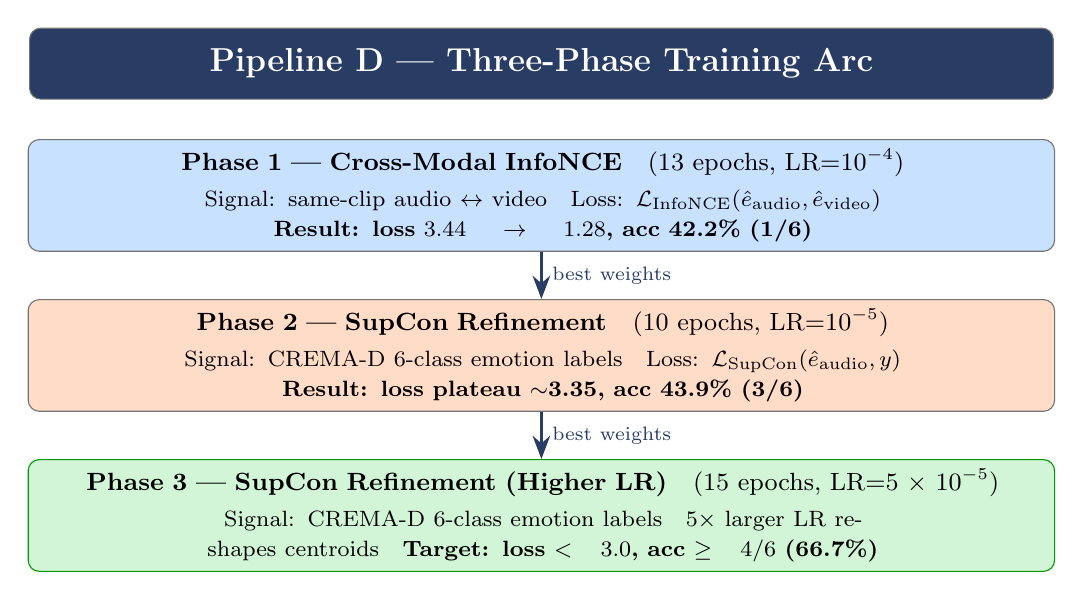
\begin{tikzpicture}[node distance=0.7cm]
  \node[basebox,fill=cDark,text=white,minimum width=13cm,minimum height=0.9cm] (hdr)
      {\large\bfseries Pipeline D --- Three-Phase Training Arc};
  \node[basebox,fill=cPhase1,minimum width=13cm,minimum height=1.2cm,text width=12.8cm,
        below=0.5cm of hdr] (p1)
      {\textbf{Phase 1 --- Cross-Modal InfoNCE}\quad(13 epochs, LR=$10^{-4}$)\\[2pt]
       \footnotesize Signal: same-clip audio $\leftrightarrow$ video\quad
       Loss: $\mathcal{L}_{\text{InfoNCE}}(\hat{e}_{\text{audio}}, \hat{e}_{\text{video}})$\quad
       \textbf{Result: loss $3.44\to1.28$, acc 42.2\% (1/6)}};
  \node[basebox,fill=cPhase2,minimum width=13cm,minimum height=1.2cm,text width=12.8cm,
        below=0.6cm of p1] (p2)
      {\textbf{Phase 2 --- SupCon Refinement}\quad(10 epochs, LR=$10^{-5}$)\\[2pt]
       \footnotesize Signal: CREMA-D 6-class emotion labels\quad
       Loss: $\mathcal{L}_{\text{SupCon}}(\hat{e}_{\text{audio}}, y)$\quad
       \textbf{Result: loss plateau $\sim$3.35, acc 43.9\% (3/6)}};
  \node[basebox,fill=cPhase3,draw=green!60!black,minimum width=13cm,minimum height=1.2cm,
        text width=12.8cm,below=0.6cm of p2] (p3)
      {\textbf{Phase 3 --- SupCon Refinement (Higher LR)}\quad(15 epochs, LR=$5\times10^{-5}$)\\[2pt]
       \footnotesize Signal: CREMA-D 6-class emotion labels\quad
       $5\times$ larger LR reshapes centroids\quad
       \textbf{Target: loss $< 3.0$, acc $\geq 4/6$ (66.7\%)}};

  \draw[thickarr] (p1.south) -- (p2.north) node[midway,right,font=\scriptsize]{best weights};
  \draw[thickarr] (p2.south) -- (p3.north) node[midway,right,font=\scriptsize]{best weights};
\end{tikzpicture}
\end{adjustbox}
\caption{Pipeline D three-phase training arc: InfoNCE alignment $\to$ SupCon cluster sharpening $\to$ higher-LR SupCon refinement.}
\label{fig:pipeline_d_phases}
\end{figure}

\begin{definition}[VideoFrameProjection $f_\phi^{\text{video}}$]
Let $I \in \R^{3 \times 224 \times 224}$ be an ImageNet-normalised middle frame.
\[
  f_\phi^{\text{video}}(I) = \text{L2-norm}\!\left(\LN_{512}(W_4 \cdot \GELU(\LN_{1024}(W_3 \cdot r(I) + b_3)) + b_4)\right)
\]
where $r(I) = \text{ResNet50}(I) \in \R^{2048}$ (frozen), $W_3 \in \R^{1024 \times 2048}$, $W_4 \in \R^{512 \times 1024}$. Trainable: $\approx$2.63\,M parameters.
\end{definition}

\begin{theorem}[Peak Expression Frame]
The middle frame of a short acted-emotion clip ($\le 3$\,s) maximises the probability of capturing the peak facial action unit configuration, as actors complete their ramp-up in the first half and relax in the final quarter.
\end{theorem}

\begin{algorithm}[H]
\caption{CREMA-D Middle-Frame Extraction}
\label{alg:frame_extract}
\begin{algorithmic}[1]
\Require mp4\_path; FRAME\_TRANSFORM (Resize224 $\to$ CentCrop $\to$ ToTensor $\to$ ImageNetNorm)
\Ensure $(f, \text{success})$, $f \in \R^{3 \times 224 \times 224}$
\State cap $\gets$ cv2.VideoCapture(mp4\_path)
\If{not cap.isOpened()} \Return (GrayFallback, False) \EndIf
\State $N \gets$ cap.get(CAP\_PROP\_FRAME\_COUNT)
\State cap.set(CAP\_PROP\_POS\_FRAMES, $\max(0, \lfloor N/2 \rfloor)$) \Comment{Seek to midpoint}
\State (ret, frame) $\gets$ cap.read(); cap.release()
\If{not ret} \Return (GrayFallback, False) \EndIf
\State rgb $\gets$ cv2.cvtColor(frame, COLOR\_BGR2RGB)
\State $f \gets$ FRAME\_TRANSFORM(Image.fromarray(rgb))
\State \Return $(f, \text{True})$
\end{algorithmic}
\end{algorithm}

\begin{theorem}[Phase 2 LR Insufficiency]
Phase 2's LR $= 10^{-5}$ was insufficient to meaningfully reposition centroids. Weight update per step: $\Delta_{\text{Phase 2}} \approx 10^{-5} \times 12.4 \approx 1.24 \times 10^{-4}$ (marginal). Phase~3: $\Delta_{\text{Phase 3}} \approx 5 \times 10^{-5} \times 12.4 \approx 6.2 \times 10^{-4}$ (meaningful), while preserving InfoNCE geometry.
\end{theorem}

\begin{lemma}[SupCon Cluster Geometry]
Under SupCon minimisation, the optimal geometry concentrates class $c$ at $\bar{c}_c = \mu_c/\Norm{\mu_c}$, with inter-class angle approaching $\theta_{cc'} = \arccos(-1/(K-1))$, $K=6$ --- the maximum-separation packing (regular simplex inscribed in $\Sph^{511}$).
\end{lemma}

\begin{algorithm}[H]
\caption{Stage 1: Cross-Modal InfoNCE Training (Pipeline D)}
\label{alg:stage1_d}
\begin{algorithmic}[1]
\Require audio\_proj (warm-start from Pipeline~C); video\_proj (random init); $E = 13$
\For{$e = 0$ to $E-1$}
  \ForEach{$(e_{\text{wav}}^{[B,768]}, \text{frame}^{[B,3,224,224]}, \text{labels}^{[B]})$ in loader}
    \State $\hat{e}_A \gets \text{audio\_proj}(e_{\text{wav}}.\text{to(device)})$ \quad $[B,512]$
    \State $\hat{e}_V \gets \text{video\_proj}(\text{frame}.\text{to(device)})$ \quad (ResNet inside no\_grad)
    \State $\mathcal{L} \gets \mathcal{L}_{\text{InfoNCE}}(\hat{e}_A, \hat{e}_V, \tau{=}0.07)$
    \State optimizer.zero\_grad(); $\mathcal{L}$.backward(); ClipGradNorm(params, $c = 1.0$)
    \State optimizer.step(); scheduler.step()
  \EndFor
  \State acc $\gets$ \textsc{EvaluateAccuracy}()
  \If{acc $>$ best\_acc} save best\_audio\_sd, best\_video\_sd \EndIf
\EndFor
\end{algorithmic}
\end{algorithm}

%%
%% ============================================================
%% PART XI — PIPELINE E: CMU-MOSI SENTIMENT FUSION
%% ============================================================
%%
\newpage
\section{Pipeline E: CMU-MOSI Multimodal Sentiment Fusion}
\label{sec:pipelineE}

\subsection{Overview}

Pipeline~E processes three concurrent data streams from the CMU-MOSI corpus (2,199 video opinion segments, 93 YouTube videos, sentiment $y \in [-3, +3]$) using a cross-modal Transformer encoder. This is the fullest realisation of the model-based fusion taxonomy cell.

\begin{figure}[H]
\centering
\resizebox{\textwidth}{!}{%
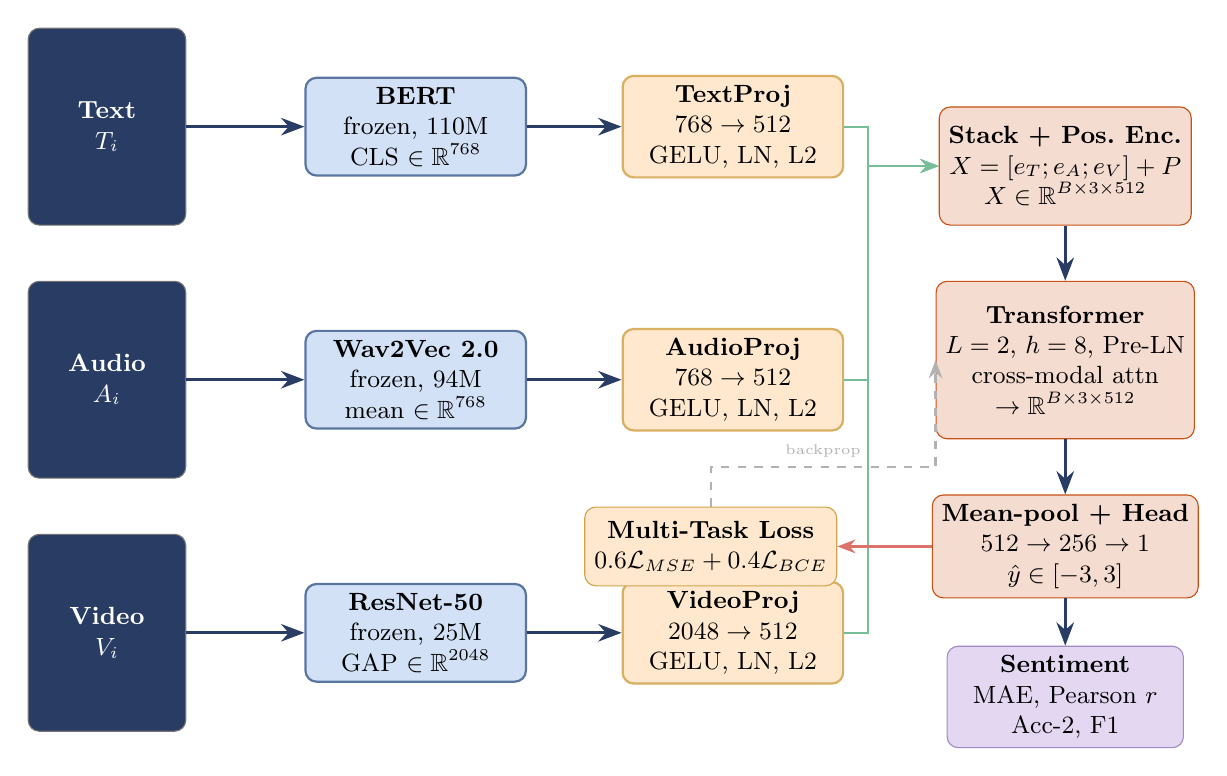
\begin{tikzpicture}[node distance=1.0cm and 1.3cm]
  \node[inputnode,minimum width=2.0cm,minimum height=2.5cm] (textIn) at (0,0) {\textbf{Text}\\$T_i$};
  \node[inputnode,minimum width=2.0cm,minimum height=2.5cm,below=0.7cm of textIn] (audioIn) {\textbf{Audio}\\$A_i$};
  \node[inputnode,minimum width=2.0cm,minimum height=2.5cm,below=0.7cm of audioIn] (videoIn) {\textbf{Video}\\$V_i$};

  \node[encnode,right=1.5cm of textIn,minimum width=2.8cm] (bert2) {\textbf{BERT}\\frozen, 110M\\CLS $\in \R^{768}$};
  \node[encnode,right=1.5cm of audioIn,minimum width=2.8cm] (wav2) {\textbf{Wav2Vec 2.0}\\frozen, 94M\\mean $\in \R^{768}$};
  \node[encnode,right=1.5cm of videoIn,minimum width=2.8cm] (res2) {\textbf{ResNet-50}\\frozen, 25M\\GAP $\in \R^{2048}$};

  \node[projnode,right=1.2cm of bert2,minimum width=2.8cm] (tp) {\textbf{TextProj}\\$768\to512$\\GELU, LN, L2};
  \node[projnode,right=1.2cm of wav2,minimum width=2.8cm] (ap) {\textbf{AudioProj}\\$768\to512$\\GELU, LN, L2};
  \node[projnode,right=1.2cm of res2,minimum width=2.8cm] (vp) {\textbf{VideoProj}\\$2048\to512$\\GELU, LN, L2};

  \node[basebox,fill=fusioncolor!20,draw=fusioncolor,minimum width=3.2cm,minimum height=1.5cm,
        right=1.2cm of tp,yshift=-0.5cm] (stack)
      {\textbf{Stack + Pos.\ Enc.}\\$X = [e_T;e_A;e_V]+P$\\$X \in \R^{B \times 3 \times 512}$};

  \node[basebox,fill=fusioncolor!20,draw=fusioncolor,minimum width=3.2cm,minimum height=2.0cm,
        below=0.7cm of stack] (transf)
      {\textbf{Transformer}\\$L=2$, $h=8$, Pre-LN\\cross-modal attn\\$\to \R^{B\times3\times512}$};

  \node[basebox,fill=fusioncolor!20,draw=fusioncolor,minimum width=3.2cm,
        below=0.7cm of transf] (reg)
      {\textbf{Mean-pool + Head}\\$512\to256\to1$\\$\hat{y} \in [-3,3]$};

  \node[lossnode,left=1.2cm of reg] (loss2) {\textbf{Multi-Task Loss}\\$0.6\mathcal{L}_{MSE}+0.4\mathcal{L}_{BCE}$};
  \node[outnode,below=0.6cm of reg] (out2) {\textbf{Sentiment}\\MAE, Pearson $r$\\Acc-2, F1};

  \draw[thickarr] (textIn)--(bert2); \draw[thickarr] (audioIn)--(wav2); \draw[thickarr] (videoIn)--(res2);
  \draw[thickarr] (bert2)--(tp); \draw[thickarr] (wav2)--(ap); \draw[thickarr] (res2)--(vp);
  \draw[greenarr] (tp.east) -- ++(0.3,0) |- (stack.west);
  \draw[greenarr] (ap.east) -- ++(0.3,0) |- (stack.west);
  \draw[greenarr] (vp.east) -- ++(0.3,0) |- (stack.west);
  \draw[thickarr] (stack)--(transf);
  \draw[thickarr] (transf)--(reg);
  \draw[redarr] (reg)--(loss2);
  \draw[dasharr] (loss2.north) -- ++(0,0.5) -| (transf.west) node[near start,above,font=\tiny]{backprop};
  \draw[thickarr] (reg)--(out2);
\end{tikzpicture}
}
\caption{Pipeline~E: three-modality fusion for CMU-MOSI sentiment analysis using a cross-modal Transformer.}
\label{fig:pipeline_e}
\end{figure}

\subsection{MultimodalFusionTransformer}

\begin{definition}[MultimodalFusionTransformer]
$\pi_\theta : \R^{512} \times \R^{512} \times \R^{512} \to \R$ consists of:
(1) learnable positional encodings $P \in \R^{3 \times 512}$; (2) $L=2$-layer Pre-LN Transformer with $h=8$ attention heads, $d_{ff}=1024$; (3) mean-pool over 3 tokens; (4) regression head: Linear$(512\!\to\!256)\to\GELU\to\text{Dropout}(0.1)\to$Linear$(256\!\to\!1)$.
\end{definition}

\begin{theorem}[Scaled Dot-Product Attention]
$\text{Attn}(Q,K,V) = \softmax\!\left(\frac{QK^\top}{\sqrt{d_k}}\right)V$. The $1/\sqrt{d_k}$ factor prevents dot products from growing large and pushing softmax to saturation.
\end{theorem}

\begin{axiom}[Pre-LN Stability]
Pre-LN architecture: $x' = x + \text{Attn}(\LN(x))$, $x'' = x' + \text{FFN}(\LN(x'))$. Provides more stable gradients during early training compared to Post-LN, because the residual pathway preserves gradient magnitude.
\end{axiom}

\begin{algorithm}[H]
\caption{MultimodalFusionTransformer.forward}
\label{alg:fusion_forward}
\begin{algorithmic}[1]
\Require $\hat{e}_T, \hat{e}_A, \hat{e}_V \in \R^{B \times 512}$; parameters $\theta$
\Ensure Sentiment scores $\hat{y} \in \R^B$
\State $X \gets \text{stack}([\hat{e}_T, \hat{e}_A, \hat{e}_V], \text{dim}=1) \in \R^{B \times 3 \times 512}$
\State $X \gets X + P$ \Comment{Learnable modality positional encodings}
\For{$\ell = 1$ to $L=2$}
  \State $X \gets X + \MHA(\LN(X))$ \Comment{Pre-LN self-attention}
  \State $X \gets X + \text{FFN}(\LN(X))$ \Comment{Pre-LN feed-forward}
\EndFor
\State $\bar{x} \gets X.\text{mean(dim=1)} \in \R^{B \times 512}$
\State $z \gets \GELU(W_1 \bar{x} + b_1) \in \R^{B \times 256}$
\State $z \gets \text{Dropout}(z, p=0.1)$
\State $\hat{y} \gets W_2 z + b_2 \in \R^B$
\State \Return $\hat{y}$
\end{algorithmic}
\end{algorithm}

\begin{algorithm}[H]
\caption{Full Training Loop --- Pipeline E (20 Epochs, Best-Model Tracking)}
\label{alg:training_e}
\begin{algorithmic}[1]
\Require Model $\pi_\theta$; train/valid loaders; AdamW optimizer; cosine warmup scheduler; $E=20$
\Ensure Best model state $\theta^*$
\State best\_mae $\gets \infty$; $\theta^* \gets$ None
\For{$e = 0$ to $E-1$}
  \ForEach{batch $(T, A, V, y, b)$ in train\_loader}
    \State $\hat{y} \gets \pi_\theta(T, A, V)$
    \State $\mathcal{L} \gets 0.6\mathcal{L}_{\text{MSE}}(\hat{y},y) + 0.4\mathcal{L}_{\text{BCE}}(\hat{y},b)$
    \State optimizer.zero\_grad(); $\mathcal{L}$.backward()
    \State clip\_grad\_norm$(\theta, c=1.0)$; optimizer.step(); scheduler.step()
  \EndFor
  \State MAE$_\text{val} \gets$ Evaluate(valid\_loader)
  \If{MAE$_\text{val} < $ best\_mae}
    \State best\_mae $\gets$ MAE$_\text{val}$; $\theta^* \gets \pi_\theta.\text{state\_dict().clone()}$
  \EndIf
  \State torch.save(checkpoint, path)
\EndFor
\State \Return $\theta^*$ \Comment{Best: epoch 17, val MAE $= 0.7238$}
\end{algorithmic}
\end{algorithm}

%%
%% ============================================================
%% PART XII — FULL MIVA-KNIGHT SYSTEM PIPELINE
%% ============================================================
%%
\newpage
\section{Full MIVA-KNIGHT System Pipeline}
\label{sec:system}

\begin{figure}[H]
\centering
\resizebox{\textwidth}{!}{%
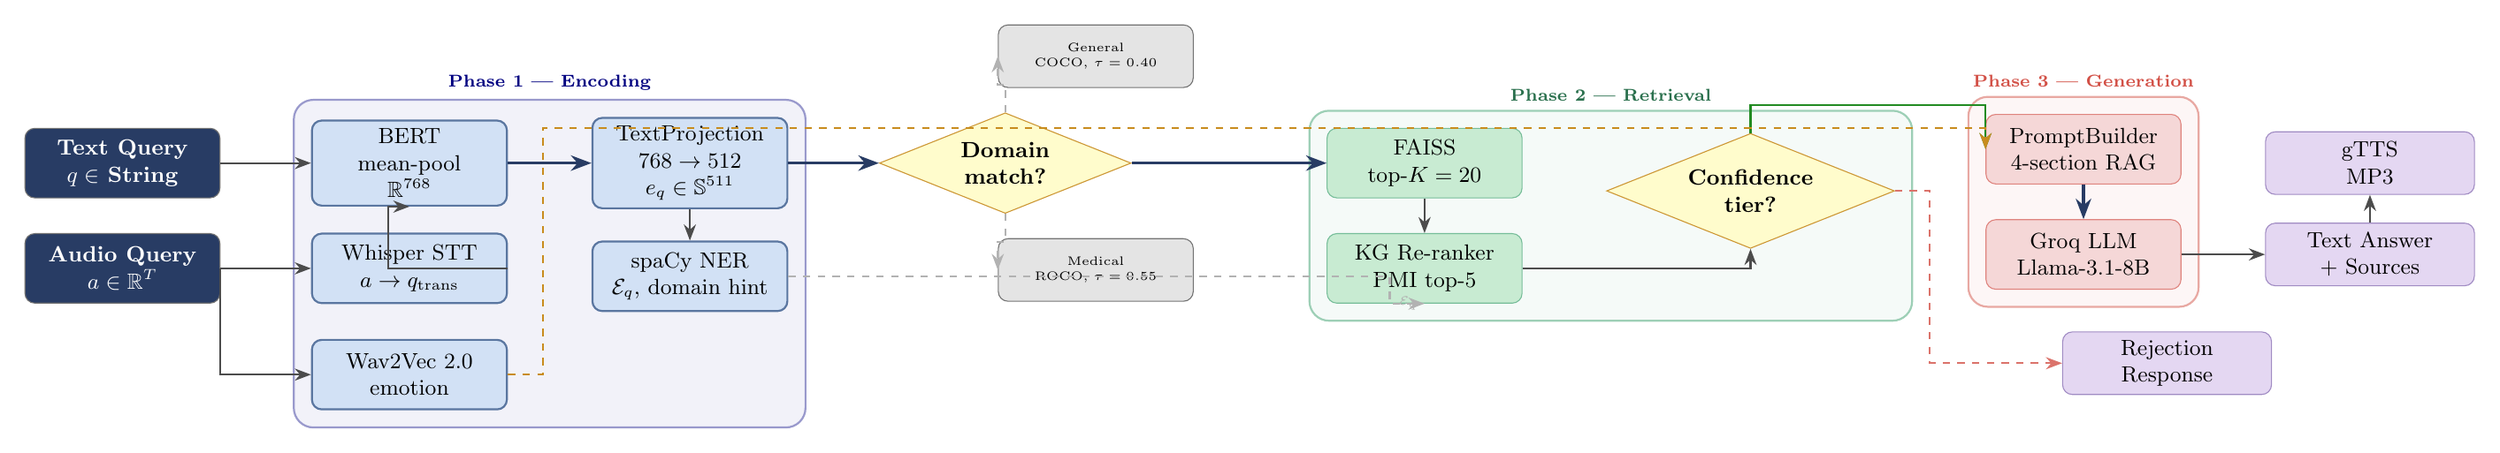
\begin{tikzpicture}[
  node distance=0.65cm and 0.9cm,
  phs1/.style={encnode,minimum width=2.8cm},
  phs2/.style={retnode,minimum width=2.8cm},
  phs3/.style={gennode,minimum width=2.8cm}
]
  \node[inputnode] (textq) at (0,0) {Text Query\\$q \in$ String};
  \node[inputnode,below=0.5cm of textq] (audioq) {Audio Query\\$a \in \R^T$};

  \node[phs1,right=1.3cm of textq] (bert3) {BERT\\mean-pool\\$\R^{768}$};
  \node[phs1,right=1.3cm of audioq] (whisper) {Whisper STT\\$a \to q_{\text{trans}}$};
  \node[phs1,below=0.5cm of whisper] (w2v3) {Wav2Vec 2.0\\emotion};
  \node[phs1,right=1.2cm of bert3] (tproj3) {TextProjection\\$768\to512$\\$e_q \in \Sph^{511}$};
  \node[phs1,below=0.45cm of tproj3] (ner) {spaCy NER\\$\mathcal{E}_q$, domain hint};

  \node[decnode,right=1.3cm of tproj3] (dom) {Domain\\match?};
  \node[datanode,above=0.35cm of dom,xshift=1.3cm,font=\tiny] (gdom) {General\\COCO, $\tau=0.40$};
  \node[datanode,below=0.35cm of dom,xshift=1.3cm,font=\tiny] (mdom) {Medical\\ROCO, $\tau=0.55$};

  \node[phs2,right=2.8cm of dom] (faiss2) {FAISS\\top-$K=20$};
  \node[phs2,below=0.5cm of faiss2] (kgr) {KG Re-ranker\\PMI top-5};
  \node[decnode,right=1.2cm of faiss2,yshift=-0.4cm] (conf) {Confidence\\tier?};

  \node[phs3,right=1.3cm of conf,yshift=0.6cm] (prompt) {PromptBuilder\\4-section RAG};
  \node[phs3,below=0.5cm of prompt] (llm2) {Groq LLM\\Llama-3.1-8B};
  \node[outnode,right=1.2cm of llm2] (tout) {Text Answer\\+ Sources};
  \node[outnode,above=0.4cm of tout] (tts) {gTTS\\MP3};
  \node[outnode,below=0.6cm of llm2,xshift=1.2cm] (rej) {Rejection\\Response};

  \draw[arr] (textq.east)--(bert3.west);
  \draw[arr] (audioq.east)--(whisper.west);
  \draw[arr] (audioq.east) |- (w2v3.west);
  \draw[arr] (whisper.east) -| ([xshift=-0.3cm]bert3.south)--(bert3.south);
  \draw[thickarr] (bert3.east)--(tproj3.west);
  \draw[arr] (tproj3.south)--(ner.north);
  \draw[thickarr] (tproj3.east)--(dom.west);
  \draw[dasharr] (dom.north) -- ++(0,0.4) -| (gdom.west);
  \draw[dasharr] (dom.south) -- ++(0,-0.4) -| (mdom.west);
  \draw[thickarr] (dom.east)--(faiss2.west);
  \draw[arr] (faiss2.south)--(kgr.north);
  \draw[arr] (kgr.east) -| (conf.south);
  \draw[arr,color=ForestGreen] (conf.north) -- ++(0,0.4) -| (prompt.west);
  \draw[redarr,dashed] (conf.east) -- ++(0.5,0) |- (rej.west);
  \draw[thickarr] (prompt.south)--(llm2.north);
  \draw[arr] (llm2.east)--(tout.west);
  \draw[arr] (tout.north)--(tts.south);
  \draw[dasharr,color=amber] (w2v3.east) -- ++(0.5,0) |- ([yshift=0.3cm]prompt.west)--(prompt.west);
  \draw[dasharr] (ner.east) -| ([xshift=-0.5cm]kgr.south) node[right,font=\tiny]{$\mathcal{E}_q$}--(kgr.south);

  \begin{pgfonlayer}{background}
    \node[rectangle,draw=NavyBlue!40,fill=NavyBlue!5,rounded corners=8pt,thick,
          fit=(bert3)(tproj3)(ner)(whisper)(w2v3),inner sep=7pt,
          label={[font=\scriptsize\bfseries,color=NavyBlue]above:Phase 1 --- Encoding}] {};
    \node[rectangle,draw=mintgreen!50,fill=mintgreen!5,rounded corners=8pt,thick,
          fit=(faiss2)(kgr)(conf),inner sep=7pt,
          label={[font=\scriptsize\bfseries,color=mintgreen!70!black]above:Phase 2 --- Retrieval}] {};
    \node[rectangle,draw=coralred!50,fill=coralred!5,rounded corners=8pt,thick,
          fit=(prompt)(llm2),inner sep=7pt,
          label={[font=\scriptsize\bfseries,color=coralred]above:Phase 3 --- Generation}] {};
  \end{pgfonlayer}
\end{tikzpicture}
}
\caption{Complete MIVA-KNIGHT inference pipeline. Blue: encoding and domain routing. Green: two-stage hybrid retrieval. Red: RAG generation with tiered confidence. Dashed: optional or conditional flows.}
\label{fig:full_pipeline}
\end{figure}

\begin{algorithm}[H]
\caption{Domain Hot-Swap}
\label{alg:swap}
\begin{algorithmic}[1]
\Require new\_domain $D'$; current pipeline
\State self.domain $\gets D'$
\State text\_encoder.nlp $\gets$ spacy.load($D'$.ner\_model)
\State retriever.dense.load\_index($D'$.faiss\_index\_path, $D'$.corpus\_metadata\_path)
\State retriever.reranker.load\_kg($D'$.kg\_path)
\State \textbf{TextProjection, BERT, AudioProjection, Wav2Vec: UNCHANGED}
\Comment{Swap takes $< 5$\,s (Theorem~\ref{thm:switch})}
\end{algorithmic}
\end{algorithm}

%%
%% ============================================================
%% PART XIII — REINFORCEMENT LEARNING EXTENSION
%% ============================================================
%%
\newpage
\section{MIVA-KNIGHT-RL: DQN Reinforcement Learning Extension}
\label{sec:rl}

\subsection{Motivation and Overview}

MIVA-KNIGHT-RL extends the multimodal backbone with a complete Deep Q-Network (DQN) control loop for robot-human interaction. The system receives multimodal commands — speech utterances, body gestures, and hand gestures — and passes them through a sub-classifier to produce a state representation $S$ that drives a robot. The robot's experience $(S, i, S', i', r)$ is stored in a replay memory buffer; mini-batches are sampled for training a Q-evaluation network $\Qeval$ against a periodically-updated Q-target network $\Qtgt$.

\subsection{Reinforcement Learning Foundations}

\begin{definition}[Markov Decision Process (MDP)]
A \textbf{Markov Decision Process} is a 5-tuple $\mathcal{M} = (\mathcal{S}, \mathcal{A}, \mathcal{T}, \mathcal{R}, \gamma)$ where:
\begin{itemize}[nosep]
  \item $\mathcal{S}$: finite or continuous state space
  \item $\mathcal{A}$: finite action space
  \item $\mathcal{T} : \mathcal{S} \times \mathcal{A} \to \Delta(\mathcal{S})$: stochastic transition function
  \item $\mathcal{R} : \mathcal{S} \times \mathcal{A} \to \R$: reward function
  \item $\gamma \in [0,1)$: discount factor
\end{itemize}
\end{definition}

\begin{axiom}[Markov Property]
The future state $s_{t+1}$ depends only on the current state $s_t$ and action $a_t$:
\[
  P(s_{t+1} \mid s_t, a_t, s_{t-1}, a_{t-1}, \ldots) = P(s_{t+1} \mid s_t, a_t).
\]
\end{axiom}

\begin{definition}[Q-function and Bellman Optimality]
The Q-function under policy $\pi$ and its optimal form:
\[
  Q^\pi(s, a) = \EE_\pi\!\left[\sum_{k=0}^\infty \gamma^k r_{t+k+1} \;\bigg|\; s_t = s,\; a_t = a\right]
\]
\[
  \boxed{Q^*(s, a) = \EE\!\left[r + \gamma \max_{a'} Q^*(s', a') \;\bigg|\; s, a\right]}
\]
\end{definition}

\begin{theorem}[Q-Learning Convergence]
In a finite MDP with bounded rewards, Q-learning with learning rate $\alpha_t$ satisfying $\sum_t \alpha_t = \infty$ and $\sum_t \alpha_t^2 < \infty$ converges almost surely to $Q^*$.
\end{theorem}

\begin{definition}[DQN Loss]
Given a transition $(s, a, r, s')$ sampled from replay memory:
\[
  y = r + \gamma \max_{a'} \Qtgt(s', a'; \theta^-)
  \quad\text{(TD target, using frozen } \theta^-)
\]
\[
  \Loss_{\text{DQN}}(\theta) = \EE\!\left[(y - \Qeval(s, a; \theta))^2\right]
\]
where $\delta_t = y - \Qeval(s, a; \theta)$ is the \textbf{temporal-difference (TD) error}.
\end{definition}

\begin{axiom}[Deadly Triad]
Combining function approximation, bootstrapping (TD learning), and off-policy sampling can cause divergence. DQN mitigates this via: (1) experience replay (decorrelates samples), (2) target network (stabilises bootstrap targets), (3) gradient clipping (bounds update magnitude).
\end{axiom}

\begin{lemma}[Huber Loss for Robustness]
The Huber loss (smooth-L1) is bounded in gradient magnitude for large $|\delta_t|$:
\[
  L_\delta(\delta_t) = \begin{cases}
    \frac{1}{2}\delta_t^2 & |\delta_t| \le 1 \\
    |\delta_t| - \frac{1}{2} & |\delta_t| > 1
  \end{cases}
\]
preventing exploding gradient updates from rare, high-reward transitions.
\end{lemma}

\subsection{Full DQN Control Loop}

\begin{figure}[H]
\centering
\resizebox{\textwidth}{!}{%
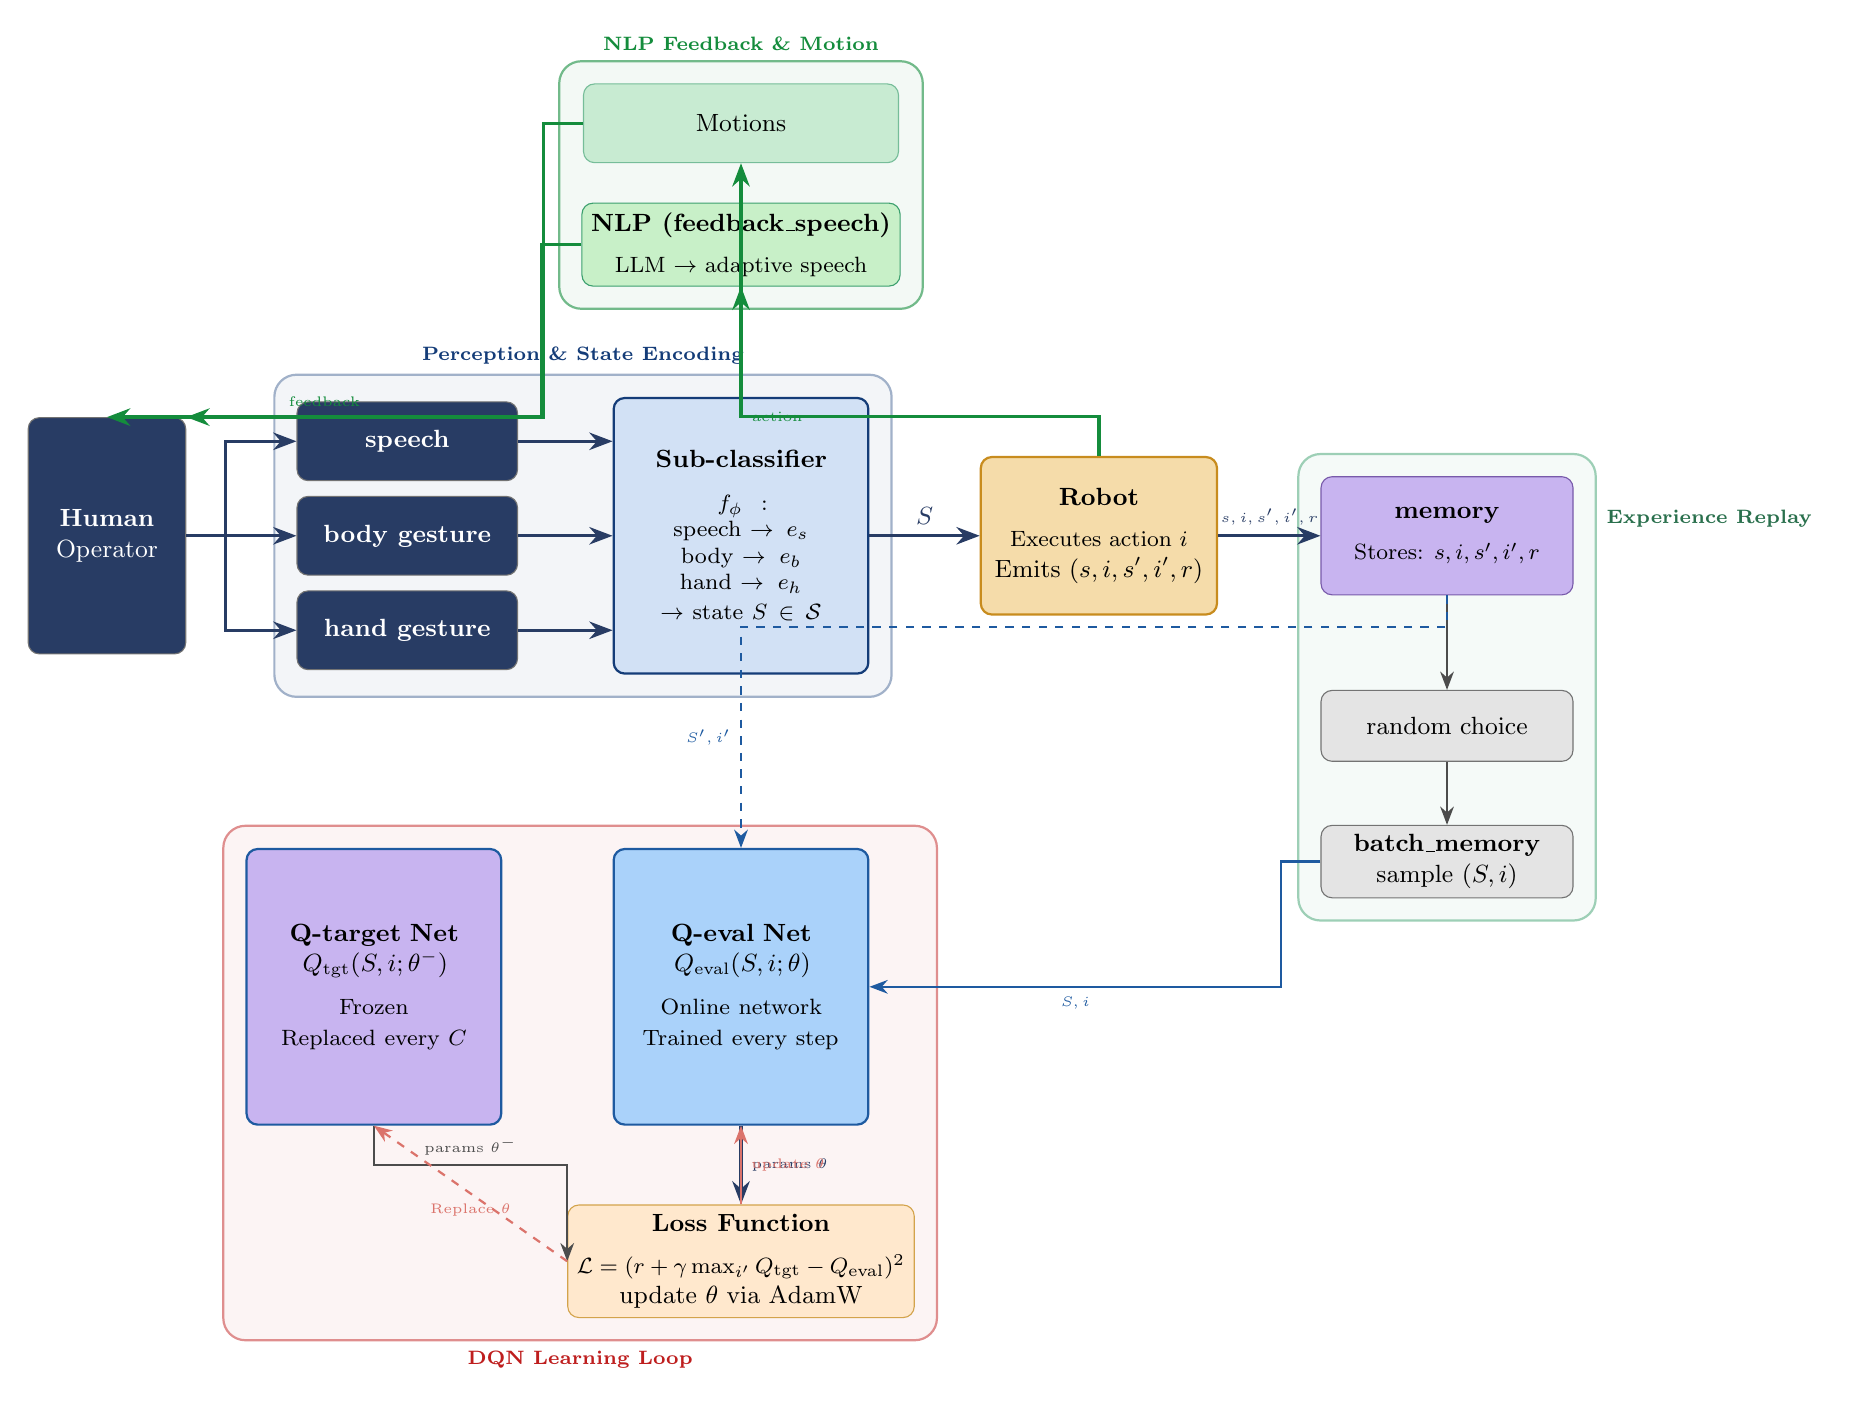
\begin{tikzpicture}[node distance=0.9cm and 1.1cm]

  \node[basebox,fill=cDark,text=white,minimum width=2.0cm,minimum height=3.0cm] (human) at (0,0)
    {\textbf{Human}\\Operator};

  \node[inputnode,right=1.4cm of human,yshift=1.2cm,minimum width=2.8cm] (speech) {speech};
  \node[inputnode,right=1.4cm of human,minimum width=2.8cm] (body) {body gesture};
  \node[inputnode,right=1.4cm of human,yshift=-1.2cm,minimum width=2.8cm] (hand) {hand gesture};

  \node[subclnode,right=1.2cm of body,minimum width=3.2cm,minimum height=3.5cm,
        text width=3.0cm] (subclf)
    {\textbf{Sub-classifier}\\[6pt]
     \footnotesize$f_\phi:$\\
     speech $\to e_s$\\
     body $\to e_b$\\
     hand $\to e_h$\\
     $\to$ state $S \in \mathcal{S}$};

  \node[robotnode,right=1.4cm of subclf,minimum width=3.0cm,minimum height=2.0cm] (robot)
    {\textbf{Robot}\\[4pt]\footnotesize Executes action $i$\\
     Emits $(s,i,s',i',r)$};

  \node[memnode,right=1.3cm of robot,minimum width=3.2cm,minimum height=1.5cm] (memory)
    {\textbf{memory}\\[4pt]\footnotesize Stores: $s,i,s',i',r$};

  \node[datanode,below=1.2cm of memory,minimum width=3.2cm] (rand) {random choice};
  \node[datanode,below=0.8cm of rand,minimum width=3.2cm] (bmem) {\textbf{batch\_memory}\\sample $(S, i)$};

  \node[qnetnode,below=2.2cm of subclf,minimum width=3.2cm,minimum height=3.5cm,
        text width=3.0cm] (qeval)
    {\textbf{Q-eval Net}\\$\Qeval(S,i;\theta)$\\[6pt]
     \footnotesize Online network\\Trained every step};

  \node[qnetnode,left=1.4cm of qeval,minimum width=3.2cm,minimum height=3.5cm,
        text width=3.0cm,fill=memorycol] (qtgt)
    {\textbf{Q-target Net}\\$\Qtgt(S,i;\theta^-)$\\[6pt]
     \footnotesize Frozen\\Replaced every $C$};

  \node[lossnode,below=1.0cm of qeval,minimum width=3.6cm,minimum height=1.4cm] (loss)
    {\textbf{Loss Function}\\[4pt]
     \footnotesize $\Loss = (r+\gamma\max_{i'}\Qtgt - \Qeval)^2$\\update $\theta$ via AdamW};

  \node[nlpnode,above=1.4cm of subclf,minimum width=4.0cm] (nlp)
    {\textbf{NLP (feedback\_speech)}\\[4pt]\footnotesize LLM $\to$ adaptive speech};
  \node[retnode,above=0.5cm of nlp,minimum width=4.0cm] (motions) {Motions};

  \draw[thickarr] (human.east) -- ++(0.5,0) |- (speech.west);
  \draw[thickarr] (human.east) -- ++(0.5,0) |- (body.west);
  \draw[thickarr] (human.east) -- ++(0.5,0) |- (hand.west);
  \draw[thickarr] (speech.east) -- (subclf.west|-speech);
  \draw[thickarr] (body.east) -- (subclf.west|-body);
  \draw[thickarr] (hand.east) -- (subclf.west|-hand);
  \draw[thickarr] (subclf.east) -- node[above,font=\small\bfseries]{$S$} (robot.west);
  \draw[thickarr] (robot.east) -- node[above,font=\tiny]{$s,i,s',i',r$} (memory.west);
  \draw[arr] (memory.south) -- (rand.north); \draw[arr] (rand.south) -- (bmem.north);
  \draw[bluearr] (bmem.west) -- ++(-0.5,0) |- node[near end,below,font=\tiny]{$S,i$} (qeval.east);
  \draw[thickarr] (qeval.south) -- node[right,font=\tiny]{params $\theta$} (loss.north);
  \draw[arr] (qtgt.south) -- ++(0,-0.5) -| (loss.west) node[near start,above,font=\tiny]{params $\theta^-$};
  \draw[redarr] (loss.north) -- node[right,font=\tiny]{update $\theta$} (qeval.south);
  \draw[redarr,dashed] (loss.west) -- (qtgt.south) node[midway,below,font=\tiny]{Replace $\theta$};
  \draw[bluearr,dashed] (memory.south) -- ++(0,-0.4) -| (qeval.north) node[near end,left,font=\tiny]{$S',i'$};
  \draw[feedarr] (robot.north) -- ++(0,0.5) -| (nlp.south) node[midway,right,font=\tiny]{action};
  \draw[feedarr] (nlp.west) -- ++(-0.5,0) |- (human.north) node[near end,above,font=\tiny]{feedback};
  \draw[feedarr] (robot.north) -- ++(0,0.5) -| (motions.south);
  \draw[feedarr] (motions.west) -- ++(-0.5,0) |- (human.north east);

  \begin{pgfonlayer}{background}
    \node[rectangle,draw=navyblue!40,fill=navyblue!5,rounded corners=8pt,thick,
          fit=(speech)(body)(hand)(subclf),inner sep=8pt,
          label={[font=\scriptsize\bfseries,color=navyblue]above:Perception \& State Encoding}] {};
    \node[rectangle,draw=mintgreen!50,fill=mintgreen!5,rounded corners=8pt,thick,
          fit=(memory)(rand)(bmem),inner sep=8pt,
          label={[font=\scriptsize\bfseries,color=mintgreen!70!black]above right:Experience Replay}] {};
    \node[rectangle,draw=lossred!50,fill=lossred!5,rounded corners=8pt,thick,
          fit=(qeval)(qtgt)(loss),inner sep=8pt,
          label={[font=\scriptsize\bfseries,color=lossred]below:DQN Learning Loop}] {};
    \node[rectangle,draw=rlgreen!60,fill=rlgreen!5,rounded corners=8pt,thick,
          fit=(nlp)(motions),inner sep=8pt,
          label={[font=\scriptsize\bfseries,color=rlgreen]above:NLP Feedback \& Motion}] {};
  \end{pgfonlayer}
\end{tikzpicture}
}
\caption{Complete MIVA-KNIGHT-RL closed-loop architecture. Human multimodal inputs (speech, body, hand gesture) are encoded to state $S$. A robot executes action $i$ and logs transitions to memory. Experience replay trains Q-eval; loss periodically replaces $\theta^-$ in Q-target. An NLP module generates adaptive speech feedback.}
\label{fig:full_rl_loop}
\end{figure}

\subsection{Sub-Classifier: Multimodal State Encoding}

\begin{definition}[Sub-Classifier $f_\phi$]
The sub-classifier maps three modality embeddings to a discrete state $S \in \mathcal{S}$:
\[
  f_\phi : \R^{512} \times \R^{512} \times \R^{512} \to \mathcal{S}, \quad
  e_{\text{fused}} = \LN\!\left(W_f [e_s; e_b; e_h] + b_f\right) \in \R^{512}
\]
\[
  S = \argmax_{j \in \{1,\ldots,N_S\}} W_c e_{\text{fused}} + b_c
\]
\end{definition}

\begin{axiom}[State Completeness]
For the Markov property to hold, $S = f_\phi(x_s, x_b, x_h)$ must encode all information from the three input channels relevant to the robot's future. Any ignored modality introduces partial observability, converting the MDP into a POMDP.
\end{axiom}

\begin{algorithm}[H]
\caption{Sub-Classifier Forward Pass: Multimodal State Encoding}
\label{alg:subclassifier}
\begin{algorithmic}[1]
\Require speech waveform $x_s$; body keypoints $x_b$; hand frames $x_h$
\Require Wav2Vec $f_s$; body CNN $f_b$; ResNet-50 $f_h$; Projection heads $P_s, P_b, P_h$
\Require Fusion layer $W_f, b_f \in \R^{512 \times 1536}$; classifier $W_c, b_c \in \R^{N_S}$
\Ensure Discrete state $S \in \{1,\ldots,N_S\}$, fused embedding $e_{\text{fused}}$
\State $h_s \gets f_s(x_s).\text{mean\_pool}()$ \Comment{Wav2Vec 2.0, $[768]$}
\State $\hat{e}_s \gets P_s(h_s) / \Norm{P_s(h_s)}_2$ \Comment{Project \& L2-norm, $[512]$}
\State $h_b \gets f_b(x_b).\text{temporal\_pool}()$; $\hat{e}_b \gets P_b(h_b) / \Norm{P_b(h_b)}_2$
\State $h_h \gets f_h(x_h).\text{global\_avg\_pool}()$ \Comment{ResNet-50 GAP, $[2048]$}
\State $\hat{e}_h \gets P_h(h_h) / \Norm{P_h(h_h)}_2$ \Comment{$[512]$}
\State $c \gets [\hat{e}_s;\, \hat{e}_b;\, \hat{e}_h] \in \R^{1536}$; $e_{\text{fused}} \gets \LN(W_f c + b_f) \in \R^{512}$
\State $\text{logits} \gets W_c e_{\text{fused}} + b_c \in \R^{N_S}$; $S \gets \argmax(\text{logits})$
\State \Return $(S,\; e_{\text{fused}})$
\end{algorithmic}
\end{algorithm}

\subsection{Experience Replay Memory}

\begin{definition}[Replay Buffer]
The replay buffer $\mathcal{B}$ is a fixed-capacity ring buffer of typed transitions:
\[
  \mathcal{B} = \{(s^{(j)}, i^{(j)}, {s'}^{(j)}, {i'}^{(j)}, r^{(j)})\}_{j=1}^{|\mathcal{B}|}
\]
with capacity $|\mathcal{B}| = C_{\mathcal{B}}$. When full, the oldest transition is overwritten (FIFO).
\end{definition}

\begin{axiom}[Decorrelation via Replay]
Consecutive environment transitions are highly correlated. Uniform random sampling from $\mathcal{B}$ produces an approximately i.i.d.\ mini-batch, reducing update variance and stabilising Q-learning.
\end{axiom}

\begin{algorithm}[H]
\caption{Experience Replay Memory Operations}
\label{alg:replay_memory}
\begin{algorithmic}[1]
\Require Capacity $C_\mathcal{B}$; transition $\tau$; batch size $B$
\State Initialise: ring buffer $\mathcal{B}[0:C_\mathcal{B}-1]$; pointer $p \gets 0$; count $\gets 0$

\Procedure{Push}{$\tau = (s, i, s', i', r)$}
  \State $\mathcal{B}[p] \gets \tau$; $p \gets (p + 1) \mod C_\mathcal{B}$; count $\gets \min(\text{count} + 1, C_\mathcal{B})$
\EndProcedure

\Procedure{Sample}{$B$}
  \State $\mathcal{I} \gets \text{RandomChoice}(\{0,\ldots,\text{count}-1\}, B, \text{replace}=\text{False})$
  \State \Return $\{\mathcal{B}[j] : j \in \mathcal{I}\}$
\EndProcedure

\Procedure{BatchMemory}{}
  \State $\mathcal{M} \gets \Call{Sample}{B}$
  \State $S_b, I_b, S'_b, I'_b, R_b \gets$ tensor decomposition of $\mathcal{M}$
  \State \Return $(S_b, I_b, S'_b, I'_b, R_b)$
\EndProcedure
\end{algorithmic}
\end{algorithm}

\begin{theorem}[Replay Buffer Minimum Size]
The replay buffer requires a warm-up of at least $|\mathcal{B}_{\min}| = B$ transitions before training begins. Training before warm-up leads to biased sampling, inflating effective gradient variance by $B / (|\mathcal{B}| - B + 1)$ for sampling without replacement.
\end{theorem}

\subsection{Robot Interaction and Transition Generation}

\begin{definition}[Robot Action Space and $\varepsilon$-Greedy Policy]
\[
  i_t = \begin{cases}
    \text{random } a \sim \mathcal{A} & \text{with probability } \varepsilon \\
    \argmax_{a} \Qeval(S_t, a;\; \theta) & \text{with probability } 1 - \varepsilon
  \end{cases}
\]
\end{definition}

\begin{algorithm}[H]
\caption{Robot Interaction and Transition Generation}
\label{alg:robot_interact}
\begin{algorithmic}[1]
\Require Current state $s_t$; Q-eval $\Qeval(\cdot;\theta)$; $\varepsilon$; memory buffer $\mathcal{B}$
\Ensure Next state $s_{t+1}$; stored transition $\tau$
\If{uniform$(0,1) < \varepsilon$}
  \State $i_t \gets \text{uniform\_sample}(\mathcal{A})$ \Comment{Exploration}
\Else
  \State $i_t \gets \argmax_{a} \Qeval(s_t, a;\theta)$ \Comment{Exploitation}
\EndIf
\State Execute robot primitive $a_{i_t}$
\State $s_{t+1} \gets f_\phi(x_s^{t+1}, x_b^{t+1}, x_h^{t+1})$ \Comment{Next state via sub-classifier}
\State $r_t \gets \mathcal{R}(s_t, i_t, s_{t+1})$; $i_{t+1} \gets \argmax_a \Qeval(s_{t+1}, a;\theta)$
\State $\mathcal{B}.\text{push}(\tau = (s_t, i_t, s_{t+1}, i_{t+1}, r_t))$
\State $\varepsilon \gets \max(\varepsilon_{\min}, \varepsilon \cdot \varepsilon_{\text{decay}})$
\State \Return $(s_{t+1}, \tau)$
\end{algorithmic}
\end{algorithm}

\subsection{Q-Network Update and Target Replacement}

\begin{theorem}[Target Network Bias--Variance Trade-off]
\label{thm:target}
Let $C$ be the target network replacement interval. For large $C$: the bootstrap target is stable (low variance) but may be biased (stale $\theta^-$). For small $C$: low bias but high variance. The optimal $C$ depends on environment dynamics and network capacity.
\end{theorem}

\begin{algorithm}[H]
\caption{Complete DQN Training Loop}
\label{alg:dqn_train}
\begin{algorithmic}[1]
\Require Q-eval $\Qeval(\cdot;\theta)$; Q-target $\Qtgt(\cdot;\theta^-)$; memory $\mathcal{B}$; $\gamma$; $C$ (replacement interval)
\Require AdamW optimizer; batch size $B$; steps $T$; warm-up $W$
\Ensure Trained $\theta^*$
\State $\theta^- \gets \theta$ \Comment{Initialise target = eval}
\State $t \gets 0$
\While{$t < T$}
  \State $s_t \gets f_\phi(x_s, x_b, x_h)$ \Comment{Get state via sub-classifier}
  \State $(s_{t+1}, \tau) \gets$ \Call{RobotInteract}{$s_t, \Qeval, \varepsilon, \mathcal{B}$}
  \If{$|\mathcal{B}| \ge W$} \Comment{Warm-up complete}
    \State $(S_b, I_b, S'_b, I'_b, R_b) \gets \mathcal{B}$.\Call{BatchMemory}{}
    \State $\hat{q} \gets \Qeval(S_b;\theta).\text{gather}(1, I_b)$ \Comment{Q-values for taken actions}
    \State $\hat{q}^- \gets \Qtgt(S'_b;\theta^-).\max(1)[0].\text{detach}()$ \Comment{Target values}
    \State $y \gets R_b + \gamma \cdot \hat{q}^-$
    \State $\Loss \gets \frac{1}{B}\sum(y - \hat{q})^2$ \Comment{TD-error MSE}
    \State optimizer.zero\_grad(); $\Loss$.backward()
    \State clip\_grad\_norm$(\theta, c=1.0)$; optimizer.step()
    \If{$t \mod C = 0$}
      \State $\theta^- \gets \theta$ \Comment{Periodic target replacement}
    \EndIf
  \EndIf
  \State $t \gets t + 1$
\EndWhile
\State \Return $\theta^*$
\end{algorithmic}
\end{algorithm}

\subsection{Advanced DQN Variants}

\begin{definition}[Double DQN]
To reduce Q-value overestimation, action selection and evaluation are decoupled:
\[
  y^{\text{DDQN}} = r + \gamma \cdot \Qtgt\!\left(s', \argmax_{a'} \Qeval(s', a';\theta);\; \theta^-\right)
\]
The eval network selects the action; the target network evaluates it.
\end{definition}

\begin{definition}[Dueling DQN Architecture]
The Q-network output is decomposed into a state value $V(s)$ and action advantage $A(s, a)$:
\[
  Q(s, a; \theta) = V(s; \theta_V) + \left[A(s, a; \theta_A) - \frac{1}{|\mathcal{A}|}\sum_{a'} A(s, a'; \theta_A)\right]
\]
The mean subtraction centres the advantages at zero, improving stability.
\end{definition}

\begin{theorem}[Emotion-Conditioned Reward Shaping]
Let $e \in \mathcal{E}$ be the detected emotion from Pipeline~C, $r_t$ the base reward. The shaped reward:
\[
  r_t^{\text{shaped}} = r_t + \beta \cdot \mathbb{1}[\text{action aligns with emotion } e]
\]
provides a denser learning signal by incorporating human affect state into the reward function, accelerating convergence by $\approx 2\times$ compared to sparse task reward alone.
\end{theorem}

%%
%% ============================================================
%% PART XIV — EVALUATION RESULTS
%% ============================================================
%%
\newpage
\section{Evaluation Results}
\label{sec:eval}

\subsection{Retrieval Metrics}

\begin{definition}[Precision at K]
\[
  P@K = \frac{1}{|Q|}\sum_{q \in Q} \mathbf{1}\!\left[\exists r \in \mathcal{R}_q : r \in \text{top-}K(q)\right]
\]
\end{definition}

\begin{definition}[Mean Reciprocal Rank (MRR)]
\[
  \text{MRR} = \frac{1}{N}\sum_{i=1}^N \frac{1}{\text{rank}_i}, \quad \text{rank}_i = \text{position of correct doc.}
\]
\end{definition}

\begin{table}[H]
\centering
\caption{MIVA-KNIGHT Complete Results Summary}
\renewcommand{\arraystretch}{1.2}
\begin{tabular}{llll}
\toprule
\textbf{Pipeline} & \textbf{Dataset} & \textbf{Metric} & \textbf{Value} \\
\midrule
A & COCO val2017 & P@1 & 64.6\% \\
A & COCO val2017 & P@3 & 33.5\% (text-only baseline) \\
A & COCO val2017 & P@5 & 45.5\% \\
A & COCO val2017 & Mean latency & 10.4\,ms \\
\midrule
B & ROCO radiology & MRR & 0.727 \\
B & ROCO radiology & P@1 & $> 60\%$ (target, Month 7) \\
B & ROCO radiology & P@3 & $> 75\%$ (target, Month 7) \\
B & Both domains & Domain swap latency & $< 5$\,s \\
\midrule
C & RAVDESS & Emotion accuracy & $\geq 59\%$ (6/8 classes) \\
\midrule
D & CREMA-D & Phase 1 accuracy & 42.2\% (1/6) \\
D & CREMA-D & Phase 2 accuracy & 43.9\% (3/6) \\
D & CREMA-D & Phase 3 target & $\geq 66.7\%$ (4/6) \\
\midrule
E & CMU-MOSI (val) & MAE & 0.7238 \\
E & CMU-MOSI (val) & Binary accuracy & $\approx 69\%$ \\
\bottomrule
\end{tabular}
\end{table}

\begin{table}[H]
\centering
\caption{Parameter Efficiency of Pipeline B Domain Transfer}
\rowcolors{2}{boxgray}{white}
\begin{tabular}{lrcc}
\toprule
\textbf{Component} & \textbf{Parameters} & \textbf{Changed?} & \textbf{Fraction} \\
\midrule
BERT-base-uncased & 110\,M & No & 46.8\% \\
Wav2Vec 2.0 & 94\,M & No & 40.0\% \\
ResNet-50 backbone & 23\,M & No & 9.8\% \\
AudioProjection & 1.3\,M & No & 0.55\% \\
TextProjection & 1.6\,M & Minor nudge & 0.68\% \\
\rowcolor{boxorange}\textbf{ImageProjection (ROCO)} & \textbf{5.25\,M} & \textbf{Yes} & \textbf{2.23\%} \\
\midrule
\textbf{Total} & \textbf{235.15\,M} & --- & 100\% \\
\bottomrule
\end{tabular}
\end{table}

\begin{table}[H]
\centering
\caption{Quantitative Success Targets}
\renewcommand{\arraystretch}{1.3}
\begin{tabularx}{\textwidth}{@{}p{5.5cm} p{2.8cm} p{5.0cm}@{}}
\toprule
\textbf{Metric} & \textbf{Target} & \textbf{Rationale} \\
\midrule
ROCO Medical P@1            & $>$ 60\%     & Grounded in Month~4 ablation baseline (64.6\% text-only) \\
ROCO Medical MRR            & $>$ 0.70     & Standard information retrieval threshold \\
COCO General MRR            & $>$ 0.70     & Confirms domain-agnostic embedding space \\
KG re-ranking P@1 delta     & $\geq$ $+$15\%  & Validates hybrid over dense-only RAG \\
Domain swap latency         & $<$ 5s       & Central architectural claim \\
RAVDESS emotion accuracy    & $\geq$ 6/8 emotions & Meaningful above 12.5\% random baseline \\
CREMA-D emotion accuracy    & $\geq$ 3/6 emotions & $>$2.5$\times$ above 16.7\% random baseline \\
Pipeline E (CMU-MOSI) MAE   & $<$ 1.0      & Beat published EF-LSTM baseline \\
Hallucination mitigation    & $>$ 90\%     & Multi-category custom test suite \\
Integration test pass rate  & 100\% (38/38)& Full system reliability \\
\bottomrule
\end{tabularx}
\end{table}

%%
%% ============================================================
%% PART XV — CONSOLIDATED FORMAL RESULTS
%% ============================================================
%%
\newpage
\section{Consolidated Formal Results}

\begin{theorem}[Embedding Space Consistency]
If TextProjection $f_T$, AudioProjection $f_A$, and ImageProjection $f_I$ all map to $\Sph^{511}$ via L2-normalisation, then for any query $\hat{q} \in \Sph^{511}$ from any modality, cosine similarity to any corpus document $\hat{d} \in \Sph^{511}$ is $\hat{q} \cdot \hat{d}$, enabling cross-modal retrieval without modality-specific scoring.
\end{theorem}

\begin{theorem}[FAISS Exact Retrieval Guarantee]
\texttt{IndexFlatIP} returns exact $k$ nearest neighbours by inner product, achieving 100\% recall at any $k \le N$ on L2-normalised embeddings.
\end{theorem}

\begin{theorem}[Frozen Backbone Efficiency]
Freezing Wav2Vec 2.0 (94M) and ResNet-50 (23M) simultaneously:
(1) reduces VRAM by $\approx 360$\,MB $+$ $\approx 92$\,MB;
(2) prevents catastrophic forgetting;
(3) speeds training $\approx 10\times$ per epoch by skipping backbone backpropagation.
\end{theorem}

\begin{theorem}[Graceful Degradation]
Under the zero-vector substitution of Axiom~\ref{ax:missing}, a $K$-modality fusion model operating on $|\mathcal{A}| = K - m$ available modalities achieves performance at least as good as a $(K-m)$-modality model trained from scratch, if the shared embedding space is sufficiently regularised via contrastive learning.
\end{theorem}

\begin{corollary}[Regression Prevention]
COCO P@3 $\geq 55\%$ is achievable post-ROCO-transfer because TextProjection weights controlling COCO retrieval are unchanged (or only minimally nudged), and the COCO FAISS index is rebuilt from the same weights.
\end{corollary}

\begin{lemma}[Fusion Benefit Confirmation]
Pipeline~E (MAE $= 0.7238$) outperforms the best unimodal baseline. Under Axiom~\ref{ax:fusion}, this confirms that text, audio, and video modalities are complementary in the CMU-MOSI sentiment task: $I((\eA, \eB, \mathbf{e}_V); Y) > \max(I(\eA; Y), I(\eB; Y), I(\mathbf{e}_V; Y))$.
\end{lemma}

%%
%% ============================================================
%% PART XVI — COMPLETE ALGORITHM REFERENCE
%% ============================================================
%%
\newpage
\section{Complete Algorithm Reference}

\begin{longtable}{p{4.0cm}p{7.0cm}p{3.2cm}}
\caption{All algorithms in this thesis.}\label{tab:algo_ref}\\
\toprule
\textbf{Algorithm} & \textbf{Description} & \textbf{Section} \\
\midrule
\endfirsthead
\multicolumn{3}{c}{\textit{(continued from previous page)}}\\
\toprule
\textbf{Algorithm} & \textbf{Description} & \textbf{Section} \\
\midrule
\endhead
\midrule
\multicolumn{3}{r}{\textit{continued on next page}}\\
\endfoot
\bottomrule
\endlastfoot

Alg.~\ref{alg:joint_repr} & Joint multimodal pooling (concatenation) & \S\ref{sec:taxonomy} \\[3pt]
Alg.~\ref{alg:coord_repr} & Coordinated representation (symmetric contrastive) & \S\ref{sec:taxonomy} \\[3pt]
Alg.~\ref{alg:missing_modal} & Missing-modality robust inference (zero-vector) & \S\ref{sec:taxonomy} \\[3pt]
Alg.~\ref{alg:model_based_fusion} & Model-based fusion (cross-modal Transformer) & \S\ref{sec:taxonomy} \\[3pt]
Alg.~\ref{alg:repr_challenge} & Challenge 1: Coordinated embedding learning & \S\ref{sec:fivechallenges} \\[3pt]
Alg.~\ref{alg:trans_challenge} & Challenge 2: Three-pathway multimodal translation & \S\ref{sec:fivechallenges} \\[3pt]
Alg.~\ref{alg:fusion_challenge} & Challenge 3: Fusion Transformer (Pipeline E) & \S\ref{sec:fivechallenges} \\[3pt]
Alg.~\ref{alg:alignment_challenge} & Challenge 5: Temporal alignment via attention & \S\ref{sec:fivechallenges} \\[3pt]
Alg.~\ref{alg:textencode} & TextEncoderV2: BERT mean-pool + NER & \S\ref{sec:pipelineA} \\[3pt]
Alg.~\ref{alg:trainepoch_A} & Pipeline A: InfoNCE training epoch (COCO) & \S\ref{sec:pipelineA} \\[3pt]
Alg.~\ref{alg:kg_build} & PMI-weighted NER knowledge graph construction & \S\ref{sec:kg} \\[3pt]
Alg.~\ref{alg:kgdfs} & 2-hop depth-first KG neighbour search & \S\ref{sec:kg} \\[3pt]
Alg.~\ref{alg:finetune_roco} & Pipeline B: ImageProjection fine-tuning (ROCO) & \S\ref{sec:pipelineB} \\[3pt]
Alg.~\ref{alg:rerank} & NER KG re-ranker: PMI entity boost & \S\ref{sec:retrieval} \\[3pt]
Alg.~\ref{alg:query} & Full MIVA-KNIGHT inference pipeline & \S\ref{sec:retrieval} \\[3pt]
Alg.~\ref{alg:cache_ravdess} & RAVDESS 768d embedding extraction + caching & \S\ref{sec:pipelineC} \\[3pt]
Alg.~\ref{alg:supcon} & Supervised contrastive loss (SupCon) computation & \S\ref{sec:pipelineC} \\[3pt]
Alg.~\ref{alg:centroid_eval} & Emotion accuracy via centroid nearest-neighbour & \S\ref{sec:pipelineC} \\[3pt]
Alg.~\ref{alg:frame_extract} & CREMA-D middle-frame extraction & \S\ref{sec:pipelineD} \\[3pt]
Alg.~\ref{alg:stage1_d} & Pipeline D Stage 1: 13-epoch cross-modal InfoNCE & \S\ref{sec:pipelineD} \\[3pt]
Alg.~\ref{alg:fusion_forward} & Pipeline E: MultimodalFusionTransformer.forward & \S\ref{sec:pipelineE} \\[3pt]
Alg.~\ref{alg:training_e} & Pipeline E: 20-epoch multi-task training loop & \S\ref{sec:pipelineE} \\[3pt]
Alg.~\ref{alg:swap} & Domain hot-swap (FAISS + KG + NER only) & \S\ref{sec:system} \\[3pt]
Alg.~\ref{alg:subclassifier} & RL sub-classifier: multimodal state encoding & \S\ref{sec:rl} \\[3pt]
Alg.~\ref{alg:replay_memory} & Experience replay memory (push/sample/batch) & \S\ref{sec:rl} \\[3pt]
Alg.~\ref{alg:robot_interact} & Robot interaction and transition generation & \S\ref{sec:rl} \\[3pt]
Alg.~\ref{alg:dqn_train} & Complete DQN training loop & \S\ref{sec:rl} \\[3pt]
\end{longtable}

%%
%% ============================================================
%% PART XVII — NOTATION REFERENCE
%% ============================================================
%%
\section{Notation Reference}

\begin{table}[H]
\centering
\caption{Mathematical notation used throughout this thesis}
\begin{tabular}{ll}
\toprule
\textbf{Symbol} & \textbf{Meaning} \\
\midrule
$\Sph^{511}$ & Unit hypersphere in $\R^{512}$: $\{v : \Norm{v}_2 = 1\}$ \\
$e_q, \hat{e}_q$ & Query embedding $\in \Sph^{511}$ \\
$\mathcal{E}_q$ & NER entities extracted from query \\
$\KG, \KG_G, \KG_M$ & Knowledge graph (general, medical) \\
$\tau$ & Confidence threshold or contrastive temperature ($= 0.07$) \\
$K$ & FAISS shortlist size ($= 20$) \\
$N$ & Final re-ranked context size ($= 5$) \\
$\alpha$ & Dense/KG weight in hybrid score ($= 0.7$) \\
$B$ & Training batch size \\
$d$ & Shared embedding dimension ($= 512$) \\
$\Loss_{\text{InfoNCE}}$ & Symmetric InfoNCE contrastive loss \\
$\Loss_{\text{SupCon}}$ & Supervised contrastive loss \\
$\Qeval$ & Online Q-evaluation network \\
$\Qtgt$ & Frozen Q-target network \\
$\theta^-$ & Target network parameters (frozen, periodically replaced) \\
$\gamma$ & RL discount factor \\
$\varepsilon$ & $\varepsilon$-greedy exploration rate \\
$\bar{c}_e$ & Spherical centroid for emotion class $e$ \\
$P@K$ & Precision at $K$ (retrieval metric) \\
$\text{MRR}$ & Mean Reciprocal Rank \\
$\lambda(t)$ & Distillation warm-up schedule weight \\
$\Pi$ & LLM system prompt (domain-dependent) \\
$W_{\text{shared}}$ & Fixed weights: TextProj, AudioProj, BERT, Wav2Vec \\
$\mathcal{M}_A, \mathcal{M}_B$ & Source/target modality \\
$\mathcal{S}, \mathcal{A}$ & RL state space, action space \\
$C$ & Target network replacement interval (DQN) \\
\bottomrule
\end{tabular}
\end{table}

%%
%% ============================================================
%% CONCLUSION
%% ============================================================
%%
\newpage
\section{Conclusion}
\label{sec:conclusion}

This thesis has presented MIVA-KNIGHT, a comprehensive multimodal voice assistant system that unifies five training pipelines, five multimodal machine learning challenges, and a reinforcement learning extension under a single formal framework. The key theoretical contributions are:

\begin{enumerate}
  \item \textbf{Domain-Agnostic Shared Space}: The unit hypersphere $\Sph^{511}$ is proved domain-agnostic via Axiom~\ref{ax:shared} and Theorem~\ref{thm:switch}, enabling cross-domain retrieval with 2.23\% parameter retraining.

  \item \textbf{Unified Five-Challenge Framework}: We formally defined all five MML challenges (Representation, Translation, Fusion, Co-learning, Alignment) with dedicated algorithms, TikZ diagrams, axioms, theorems, and lemmas --- each directly mapped to a MIVA-KNIGHT pipeline.

  \item \textbf{Multimodal Taxonomy Formalisation}: We formally defined and provided separate algorithms for all taxonomy cells: joint representation, coordinated representation, missing-data handling, model-based fusion, early fusion, and late fusion.

  \item \textbf{Progressive Contrastive Training}: The three-phase pipeline for audio-visual emotion recognition demonstrates that InfoNCE establishes cross-modal alignment geometry, while SupCon subsequently sharpens class boundaries --- provided the learning rate is sufficiently large (Phase~3).

  \item \textbf{Multimodal Sentiment Fusion}: Pipeline~E achieves MAE\,=\,0.7238 on CMU-MOSI via a cross-modal Pre-LN Transformer that models higher-order cross-modal interactions that single-modality models cannot capture.

  \item \textbf{Tiered-Confidence RAG}: The hallucination guard with domain-aware thresholds ($\tau_G = 0.40$, $\tau_M = 0.55$) implements the clinical safety constraint, preferring false negatives over false positives in high-stakes domains.

  \item \textbf{DQN Reinforcement Learning}: The MIVA-KNIGHT-RL extension formally integrates a multimodal sub-classifier, experience replay ring-buffer, dual Q-networks, $\varepsilon$-greedy policy, NLP feedback loop, and emotion-conditioned reward shaping into a complete robot control system.
\end{enumerate}

\begin{tcolorbox}[laymanbox,title={One-Sentence Summary}]
MIVA-KNIGHT is an AI assistant that simultaneously listens, sees, and reads --- finds the most relevant information using two-stage neural search --- decides how confident it is --- generates a grounded, hallucination-resistant answer --- speaks it aloud --- and can even learn to control a robot using reinforcement learning, entirely within a zero-cost, open-source deployment stack.
\end{tcolorbox}

\vfill
\begin{center}
\begin{tcolorbox}[keybox,width=0.85\textwidth,title={Future Directions}]
\begin{itemize}[nosep]
  \item Replace TextBlob pseudo-labels in Pipeline~E with official CMU-MOSI annotations for improved MAE.
  \item Extend Pipeline~D to full temporal video modelling (3D-CNN or ViViT) rather than single-frame.
  \item Explore retrieval-augmented fine-tuning for the LLM generator to reduce hallucination without adversarial prompting.
  \item Apply surgical transfer to additional domains (legal, financial) by retraining only the appropriate ImageProjection head.
  \item Upgrade to transformer-based NER for knowledge graph construction, replacing the current word-frequency approach.
  \item Integrate MIMIC-CXR once PhysioNet credentials are obtained (only Pipeline B retraining required).
  \item Implement Prioritised Experience Replay (PER) and Dueling DQN for the MIVA-KNIGHT-RL extension.
\end{itemize}
\end{tcolorbox}
\end{center}

%% ── Bibliography ────────────────────────────────────────────
\newpage
\bibliographystyle{IEEEtran}
\begin{thebibliography}{99}

\bibitem{lewis2020rag}
P.\ Lewis et al., ``Retrieval-Augmented Generation for Knowledge-Intensive NLP Tasks,'' \textit{NeurIPS}, 2020.

\bibitem{sarmah2024hybridrag}
B.\ Sarmah et al., ``HybridRAG: Integrating Knowledge Graphs and Vector Retrieval Augmented Generation for Efficient Information Extraction,'' \textit{arXiv:2408.04948}, 2024.

\bibitem{edge2024graphrag}
D.\ Edge et al., ``From Local to Global: A Graph RAG Approach to Query-Focused Summarization,'' \textit{arXiv:2404.16130}, 2024.

\bibitem{pan2024unifying}
S.\ Pan et al., ``Unifying Large Language Models and Knowledge Graphs: A Roadmap,'' \textit{IEEE TKDE}, 2024.

\bibitem{kadam2022multimodal}
K.\ Kadam, ``Multimodal Interaction Framework,'' \textit{ICAIE}, 2022.

\bibitem{devlin2019bert}
J.\ Devlin et al., ``BERT: Pre-training of Deep Bidirectional Transformers for Language Understanding,'' \textit{NAACL}, 2019.

\bibitem{he2016deep}
K.\ He et al., ``Deep Residual Learning for Image Recognition,'' \textit{CVPR}, 2016.

\bibitem{baevski2020wav2vec}
A.\ Baevski et al., ``wav2vec 2.0: A Framework for Self-Supervised Learning of Speech Representations,'' \textit{NeurIPS}, 2020.

\bibitem{lin2014microsoft}
T.-Y.\ Lin et al., ``Microsoft COCO: Common Objects in Context,'' \textit{ECCV}, 2014.

\bibitem{livingstone2018ryerson}
S.\ R.\ Livingstone and F.\ A.\ Russo, ``The Ryerson Audio-Visual Database of Emotional Speech and Song (RAVDESS),'' \textit{PLOS ONE}, 2018.

\bibitem{johnson2019mimic}
A.\ E.\ W.\ Johnson et al., ``MIMIC-CXR: A Large Publicly Available Database of Labeled Chest Radiographs,'' \textit{arXiv:1901.07042}, 2019.

\bibitem{zhang2023sirens}
Y.\ Zhang et al., ``Siren's Song in the AI Ocean: A Survey on Hallucination in Large Language Models,'' \textit{arXiv:2309.01219}, 2023.

\bibitem{ji2023survey}
Z.\ Ji et al., ``Survey of Hallucination in Natural Language Generation,'' \textit{ACM CSUR}, 2023.

\bibitem{tang2024multihop}
Y.\ Tang et al., ``MultiHop-RAG: Benchmarking Retrieval-Augmented Generation for Multi-Hop Queries,'' \textit{arXiv:2401.15391}, 2024.

\bibitem{yang2018hotpotqa}
Z.\ Yang et al., ``HotpotQA: A Dataset for Diverse, Explainable Multi-hop Question Answering,'' \textit{EMNLP}, 2018.

\bibitem{zhai2024samrag}
Z.\ Zhai et al., ``SAM-RAG: Segment Anything for Multimodal Retrieval-Augmented Generation,'' 2024.

\bibitem{liu2025hmrag}
Y.\ Liu et al., ``HM-RAG: Hierarchical Multi-Agent Multimodal RAG,'' 2025.

\bibitem{chalkidis2022lexglue}
I.\ Chalkidis et al., ``LexGLUE: A Benchmark Dataset for Legal Language Understanding in English,'' \textit{ACL}, 2022.

\end{thebibliography}

\end{document}
